% !TeX program = xelatex
\documentclass[10pt,aspectratio=169,xcolor=dvipsnames]{beamer}
\usepackage[T1]{fontenc}
\usepackage{lmodern}
\renewcommand{\familydefault}{\sfdefault}
\usepackage{amsmath,amssymb,mathtools,bm}
\usepackage{booktabs,array,colortbl,multirow}
\usepackage{tikz}
\usetikzlibrary{arrows.meta,positioning,shapes.geometric,fit,backgrounds,calc}
\usepackage{xcolor}
\usepackage{siunitx}
\usepackage{pifont}
\usepackage{adjustbox}
\usepackage{listings}
\lstset{
  basicstyle=\scriptsize\ttfamily,
  keywordstyle=\color{NavyBlue}\bfseries,
  commentstyle=\color{ForestGreen!70!black},
  stringstyle=\color{BrickRed},
  showstringspaces=false,
  breaklines=true,
  columns=fullflexible,
  frame=single,
  rulecolor=\color{gray!40},
  backgroundcolor=\color{gray!5},
  xleftmargin=1mm,
  xrightmargin=1mm
}

\hfuzz=60pt
\vfuzz=60pt
\hbadness=10000
\vbadness=10000

% ------------------------------------------------------------------
% Theme - aligned with the previous slide_EN deck
% ------------------------------------------------------------------
\usetheme{metropolis}
\usecolortheme{default}
\setbeamercolor{background canvas}{bg=white}
\setbeamercolor{normal text}{bg=white,fg=black}
\ifdefined\setsansfont
  \setsansfont[NFSSFamily=lmss]{Latin Modern Sans}
  \setmonofont[NFSSFamily=lmtt]{Latin Modern Mono}
\fi
\setbeamercolor{frametitle}{bg=NavyBlue!85!black,fg=white}
\setbeamercolor{progress bar}{fg=NavyBlue}
\setbeamerfont{frametitle}{size=\large,series=\bfseries}
\setbeamertemplate{navigation symbols}{}
\setbeamercolor{block title}{bg=NavyBlue!80!black,fg=white}
\setbeamercolor{block body}{bg=NavyBlue!5!white,fg=black}
\setbeamercolor{alertblock title}{bg=BrickRed!85!black,fg=white}
\setbeamercolor{alertblock body}{bg=BrickRed!5!white,fg=black}
\setbeamercolor{exampleblock title}{bg=ForestGreen!75!black,fg=white}
\setbeamercolor{exampleblock body}{bg=ForestGreen!5!white,fg=black}

% ------------------------------------------------------------------
% Macros
% ------------------------------------------------------------------
\newcommand{\R}{\mathbb{R}}
\newcommand{\E}{\mathbb{E}}
\newcommand{\PL}{\mathrm{PL}}
\newcommand{\HPL}{\mathrm{HPL}}
\newcommand{\VPL}{\mathrm{VPL}}
\newcommand{\AL}{\mathrm{AL}}
\newcommand{\HAL}{\mathrm{HAL}}
\newcommand{\VAL}{\mathrm{VAL}}
\newcommand{\IM}{\mathrm{IM}}
\newcommand{\PI}{\mathrm{PI}}
\newcommand{\IR}{\mathrm{IR}}
\newcommand{\FIM}{\mathrm{FIM}}
\newcommand{\mon}{\mathrm{mon}}
\newcommand{\pred}{\mathrm{pred}}
\newcommand{\diag}{\mathrm{diag}}
\newcommand{\tr}{\mathrm{tr}}
\newcommand{\rank}{\mathrm{rank}}
\newcommand{\clip}{\mathrm{clip}}
\newcommand{\Interp}{\mathrm{Interp}}
\newcommand{\Occ}{\mathrm{Occ}}
\newcommand{\ESDF}{\mathrm{ESDF}}
\newcommand{\Hset}{\mathcal{H}}
\newcommand{\Fset}{\mathcal{F}}
\newcommand{\Sset}{\mathcal{S}}
\newcommand{\Cset}{\mathcal{C}}
\newcommand{\Mmap}{\mathcal{M}}
\newcommand{\Ggrid}{\mathcal{G}}
\newcommand{\innov}[1]{\textcolor{NavyBlue}{\textbf{#1}}}
\newcommand{\warn}[1]{\textcolor{BrickRed}{\textbf{#1}}}
\newcommand{\blue}[1]{\textcolor{NavyBlue}{\textbf{#1}}}
\newcommand{\green}[1]{\textcolor{ForestGreen!75!black}{\textbf{#1}}}
\newcommand{\red}[1]{\textcolor{BrickRed}{\textbf{#1}}}
\newcommand{\ok}{\textcolor{ForestGreen}{\ding{51}}}
\newcommand{\bad}{\textcolor{BrickRed}{\ding{55}}}
\newcommand{\smallvspace}{\vspace{3pt}}
\newcommand{\tightitem}{\setlength{\itemsep}{2pt}\setlength{\parskip}{0pt}\setlength{\parsep}{0pt}}
\newcommand{\smalltable}[1]{\begin{adjustbox}{max width=\linewidth}\scriptsize#1\end{adjustbox}}
\newcommand{\imageplaceholder}[2][45mm]{%
  \begin{center}
    \begin{tikzpicture}
      \node[
        draw=NavyBlue!55!black,
        rounded corners=2pt,
        fill=NavyBlue!4,
        minimum width=0.95\linewidth,
        minimum height=#1,
        align=center,
        inner sep=5pt,
        text width=0.86\linewidth
      ] {\footnotesize\textbf{Image placeholder}\par\scriptsize #2};
    \end{tikzpicture}
  \end{center}%
}

\title{Safety-Aware Navigation and Planning}

\author{Naigui Xiao}
\institute{Trustworthy AI and Autonomous Systems Laboratory\\Department of Aeronautical and Aviation Engineering}
\date{May 2026}

\begin{document}

\maketitle

\begin{frame}{Outline}
  \footnotesize
  \tableofcontents
\end{frame}

% ==================================================================
\section{Ch1 Background \& Motivation}
% ==================================================================

\begin{frame}[t]{1.1 Why Safety Is More Than Obstacle Avoidance}
  \small
  \begin{columns}[T]
    \column{0.54\textwidth}
    \textbf{Low-altitude UAV autonomy is a coupled safety problem.}
    \begin{itemize}\tightitem
      \item Perception detects obstacles in the map.
      \item Localization decides where the UAV believes itself to be.
      \item Planning avoids obstacles only for the estimated trajectory.
      \item Control tracks the reference, but cannot remove unbounded state error.
    \end{itemize}
    \begin{alertblock}{Core message}
      A UAV can be collision-free in the map but unsafe in the real world if localization uncertainty is ignored.
    \end{alertblock}

    \column{0.46\textwidth}
    \vspace{-2mm}
    
    \begin{figure}
        \centering
        
\includegraphics[width=0.8\linewidth]{pics/1.png}
        \label{fig:placeholder}
    \end{figure}
  \end{columns}
\end{frame}

\begin{frame}[t]{1.2 Forest Example: GNSS Degradation Under Canopy}
  \small
  \begin{columns}[T]
    \column{1.0\textwidth}
    \textbf{In forests, GNSS is often partially available but statistically degraded.}
    \vspace{1mm}
    \begin{itemize}\tightitem
      \item \blue{Attenuation}: foliage weakens direct signals.
      \item \blue{Multipath}: canopy, trunks, and ground create reflected paths.
      \item \blue{Visibility loss}: fewer satellites and poor angular diversity.
    \end{itemize}
    \begin{block}{Planning implication}
      Two nearby forest routes may have similar obstacle clearance but very different GNSS integrity.
    \end{block}

    % \column{1.0\textwidth}
    \begin{figure}
        \centering
        
\includegraphics[width=0.9\linewidth]{pics/2.png}
        \label{fig:placeholder}
    \end{figure}
  \end{columns}
\end{frame}

\begin{frame}[t]{1.3 Urban Canyon Example: Geometry-Dependent Integrity}
  \small
  \begin{columns}[T]
    \column{0.52\textwidth}
    \textbf{In urban canyons, the shortest route may have the weakest navigation geometry.}
    \vspace{8mm}
    
    \smalltable{%
      \begin{tabular}{p{0.18\textwidth}p{0.19\textwidth}p{0.21\textwidth}p{0.22\textwidth}}
        \toprule
        \textbf{Route} & \textbf{Distance} & \textbf{Sky view} & \textbf{Integrity}\\
        \midrule
        A & shorter & blocked / NLOS & higher risk\\
        B & longer & more open & lower risk\\
        \bottomrule
    \end{tabular}}
    \vspace{4mm}
    \begin{alertblock}{Planning implication}
      Obstacle-free path search alone cannot distinguish paths with different navigation integrity.
    \end{alertblock}

    \column{0.48\textwidth}
    \begin{figure}
        \centering
        
\includegraphics[width=0.8\linewidth]{pics/3.png}
        % \caption{Enter Caption}
        \label{fig:placeholder}
    \end{figure}
  \end{columns}
\end{frame}

\begin{frame}[t]{1.4 Collision-Free Nominal Path Is Not Enough}
  \small
  \begin{columns}[T]
    \column{0.50\textwidth}
    \begin{block}{Traditional planner assumption}
      The planner checks whether the \textbf{nominal estimated trajectory} avoids obstacles.
    \end{block}
    \begin{alertblock}{Failure mode}
      The nominal path may be outside obstacles, while the localization uncertainty tube intersects trees, walls, or other hazards.
    \end{alertblock}
    \begin{exampleblock}{Key distinction}
      \textbf{Collision-free path}: safety of the estimated trajectory.\\
      \textbf{Integrity-safe path}: safety of the possible true trajectory.
    \end{exampleblock}

    \column{0.50\textwidth}
    \begin{figure}
        \centering
        
\includegraphics[width=0.8\linewidth]{pics/5.png}
        \label{fig:placeholder}
    \end{figure}
  \end{columns}
\end{frame}

\begin{frame}[t]{1.5 From Accuracy to Integrity}
  \small
  \begin{columns}[T]
    \column{0.5\textwidth}
    \begin{alertblock}{Accuracy-oriented navigation}
      \begin{itemize}\tightitem
        \item Asks: \emph{How close is the estimate on average?}
        \item Uses RMSE, drift, and tracking error.
        \item May miss tail risk, overconfidence, and faults.
      \end{itemize}
    \end{alertblock}

    % \column{0.5\textwidth}
    \begin{exampleblock}{Integrity-oriented navigation}
      \begin{itemize}\tightitem
        \item Asks: \emph{Can the system bound its error with high confidence?}
        \item Uses protection level and alert limits.
        \item Supports safety decisions before collision risk becomes visible.
      \end{itemize}
    \end{exampleblock}
  \vspace{0.01mm}
    % \begin{figure}
    %     \centering
    %     
\includegraphics[width=0.8\linewidth]{pics/4.png}
    %     \label{fig:placeholder}
    % \end{figure}
    \column{0.50\textwidth}
    \vspace{-2mm}
    
    \begin{figure}
        \centering
        
\includegraphics[width=0.9\linewidth]{pics/6.png}
        \label{fig:placeholder}
    \end{figure}
  \end{columns}
    
\end{frame}

\begin{frame}[t]{1.6 PL and AL: A Shared Safety Language}
  \small

  % --- Top row: two side-by-side blocks ---
  \begin{columns}[T,totalwidth=\textwidth]
    \column{0.48\textwidth}
    \begin{block}{Protection Level (PL)}
      Localization-side bound on possible position error.
    \end{block}

    \column{0.48\textwidth}
    \begin{block}{Alert Limit (AL)}
      Environment-side tolerable error before collision or mission hazard.
    \end{block}
  \end{columns}

  \vspace{-2mm}

  % --- Full-width formula block ---
  \begin{center}
    \Large
    \[
      \PL < \AL
    \]
    \vspace{-6mm}
    \[
      \IM = \AL - \PL
    \]
  \end{center}

  \vspace{-1mm}

  % --- Full-width explanation ---
  \begin{itemize}\tightitem
    \item PL increases when sensing or geometry becomes weak.
    \item AL decreases near obstacles or vertical boundaries.
    \item Planning should prefer large positive integrity margin.
  \end{itemize}

  % \vspace{1mm}

  \begin{exampleblock}{Planning interpretation}
    The planner should choose trajectories that keep the localization-side risk below the environment-side tolerance.
  \end{exampleblock}

\end{frame}

\begin{frame}[t]{1.7 Why Localization and Planning Must Be Metric-Unified}
  \small
  \begin{columns}[T]
    \column{0.49\textwidth}
    \begin{alertblock}{Conventional pipeline}
      \centering Estimator $\rightarrow$ mean pose $\rightarrow$ Planner
    \end{alertblock}
    \begin{itemize}\tightitem
      \item SLAM knows uncertainty, planner does not.
      \item ARAIM can raise alarms, but cannot change the future path.
      \item Planning optimizes collision and smoothness, not localization integrity.
    \end{itemize}

    \column{0.49\textwidth}
    \begin{exampleblock}{Integrity-aware pipeline}
      \centering Estimator + ARAIM $\rightarrow$ PL/IM field $\rightarrow$ Planner
    \end{exampleblock}
    \begin{itemize}\tightitem
      \item Future trajectory avoids low-integrity regions.
      \item Certified monitoring and advisory planning remain separated.
      \item PL becomes the shared metric between localization and planning.
    \end{itemize}
  \end{columns}
  \vspace{1mm}
  \begin{block}{Positioning of this work}
    The goal is not full joint SLAM-planning optimization, but a metric-unified architecture through PL and IM.
  \end{block}
\end{frame}

% ==================================================================
\section{Ch2 Research Gaps \& Contributions}
% ==================================================================

\begin{frame}[t]{2.1 Research Gaps}
  \small
  \textbf{The missing component is a real-time, queryable integrity field that connects localization monitoring to motion planning.}
  \vspace{8mm}
  
  \smalltable{%
    \begin{tabular}{p{0.24\textwidth}p{0.34\textwidth}p{0.34\textwidth}}
      \toprule
      \textbf{Gap} & \textbf{Existing limitation} & \textbf{Consequence}\\
      \midrule
      Uncertainty discarded before planning & Planner receives the mean pose, not an integrity-aware state. & Nominally safe paths may be unsafe under localization uncertainty.\\
      Current ARAIM is not a future planner query & ARAIM monitors the current epoch and real measurements. & Alarms can come too late for proactive route selection.\\
      LiDAR integrity lacks interpretable fault units & ICP is often treated as a black-box pose factor. & Weak fault diagnosis and weak LiDAR PL explanation.\\
      No unified risk map for planning & ESDF, PL, and cost fields may be separate, duplicated, or stale. & Inconsistent A* and back-end behavior.\\
      \bottomrule
  \end{tabular}}
\end{frame}

\begin{frame}[t]{2.2 Core Research Question and Scope}
  \small
  \begin{block}{Core research question}
    How can protection level become a first-class planning signal, so that a UAV avoids low-integrity regions before integrity is lost?
  \end{block}
  \begin{columns}[T]
    \column{0.50\textwidth}
    \textbf{Sub-questions}
    \begin{enumerate}\tightitem
      \item How to monitor current GNSS--LiDAR integrity?
      \item How to predict future advisory PL over candidate positions?
      \item How to inject predicted integrity into planning in real time?
    \end{enumerate}

    \column{0.50\textwidth}
    \textbf{Scope of this work}
    \begin{itemize}\tightitem
      \item Discrete-time FGO + decoupled planning.
      \item Metric-unified through PL and IM.
      \item Current monitor remains conservative.
      \item Future prediction is advisory, not certified ARAIM.
    \end{itemize}
  \end{columns}
\end{frame}

\begin{frame}[t]{2.3 Proposed Solution Overview}
  \small
  \textbf{The proposed system separates current monitoring from future advisory planning, but connects both through the same integrity language.}
  \vspace{8mm}
  
  \smalltable{%
    \begin{tabular}{p{0.19\textwidth}p{0.73\textwidth}}
      \toprule
      \textbf{Module} & \textbf{Role}\\
      \midrule
      FGO Snapshot & Provides pose, conservative covariance, GNSS epoch, and LiDAR factor-block summaries.\\
      Current ARAIM Monitor & Computes conservative current $\PL^{\mon}$ and alarm flags from real measurements.\\
      Advisory PL Predictor & Estimates future model-based $\PL^{\pred}$ over candidate positions.\\
      PL / IM Map & Caches predicted PL, AL, IM, cost, age, and flags for fast planner query.\\
      Integrity-Aware Planner & Uses the same risk field in front-end search and back-end trajectory optimization.\\
      \bottomrule
  \end{tabular}}
  \vspace{1mm}
  {\scriptsize\color{BrickRed}\textbf{Important boundary:} $\PL^{\mon}$ is current, measurement-based, and alarm-oriented; $\PL^{\pred}$ is future, model-based, and planning-oriented.\par}
\end{frame}

\begin{frame}[t]{2.4 Contributions}
  \small
  \begin{columns}[T]
    \column{0.49\textwidth}
    \begin{block}{C1. Integrity-aware localization interface}
      \begin{itemize}\tightitem
        \item FGO snapshot exports pose, covariance, GNSS epoch, and LiDAR block summaries.
        \item The estimator becomes an integrity data provider, not only an odometry source.
      \end{itemize}
    \end{block}
    \begin{block}{C2. Current dual-source ARAIM monitor}
      \begin{itemize}\tightitem
        \item GNSS satellite / constellation fault hypotheses.
        \item LiDAR VGICP source--target--level factor-block hypotheses.
        \item Conservative current monitor fusion.
      \end{itemize}
    \end{block}

    \column{0.49\textwidth}
    \begin{block}{C3. Advisory GNSS--LiDAR PL field}
      \begin{itemize}\tightitem
        \item GNSS visibility and geometry prediction.
        \item LiDAR observability and feature-geometry prediction.
        \item Fused advisory PL / IM field for planning.
      \end{itemize}
    \end{block}
    \begin{block}{C4. Integrity-aware planning}
      \begin{itemize}\tightitem
        \item Unified risk grid for ESDF, AL, PL, IM, cost, age, and flags.
        \item A* front-end uses integrity cost.
        \item B-spline back-end queries the same field.
      \end{itemize}
    \end{block}
  \end{columns}
  \vspace{1mm}
  {\centering\color{ForestGreen}\textbf{Takeaway:} The system does not only monitor integrity; it plans with integrity.\par}
\end{frame}

\begin{frame}[t]{2.5 Transition to Methodology}
  \small
  \textbf{The rest of the talk explains how each block is implemented and validated.}
  \vspace{2mm}
  
  \smalltable{%
    \begin{tabular}{p{0.23\textwidth}p{0.62\textwidth}}
      \toprule
      \textbf{Methodology block} & \textbf{Key question}\\
      \midrule
      Localization backbone & What information must the estimator expose?\\
      Current ARAIM monitor & How is current GNSS--LiDAR PL monitored?\\
      Advisory predictor & How is future PL estimated without claiming future certified ARAIM?\\
      Predicted PL map & How is the predictor converted into a cached planner field?\\
      Planning module & How do A* and B-spline optimization use the same integrity cost?\\
      \bottomrule
  \end{tabular}}
  \vspace{2mm}
  \begin{exampleblock}{Roadmap to Ch3}
    Localization Snapshot $\rightarrow$ Current ARAIM Monitor $\rightarrow$ Advisory PL Predictor $\rightarrow$ Predicted PL/IM Map $\rightarrow$ Integrity-Aware Planner.
  \end{exampleblock}
\end{frame}

% ==================================================================
\section{Ch3 Methodology}
% ==================================================================

\begin{frame}{3.0.1 Updated Methodology Structure}
  \small
  \begin{block}{Design objective}
    The updated methodology separates \innov{current certified monitoring} from \innov{future advisory prediction}, while keeping both connected through a common position-domain metric: the protection level (PL).
  \end{block}

  \begin{columns}[T]
    \column{0.5\textwidth}
    \textbf{Main methodology modules}
    \begin{enumerate}\footnotesize
      \item \textbf{Localization backbone}: GNSS-LiDAR-IMU factor graph.
      \item \textbf{Current dual-source ARAIM}: current PL and alarm decision.
      \item \textbf{Advisory PL predictor}: future query model for candidate positions.
      \item \textbf{Predicted PL map}: rolling multi-layer field for planning.
      \item \textbf{Integrity-aware planning}: A* front-end and B-spline back-end.
    \end{enumerate}

    \column{0.5\textwidth}
    \textbf{Why this structure is necessary}
    \begin{itemize}\footnotesize
      \item ARAIM uses \textbf{real residuals} at the current epoch.
      \item Future prediction has no real residuals, so it is \textbf{advisory}.
      \item The planner needs a \textbf{dense, queryable, cached} PL/cost field.
      \item GNSS and LiDAR should be fused in \textbf{position-domain information}, not by hand-tuned risk-score addition.
    \end{itemize}
  \end{columns}
\end{frame}

\begin{frame}{3.0.2 End-to-End Workflow: Two Integrity Paths}
  \centering
  % \resizebox{0.96\textwidth}{!}{%
  %   \begin{tikzpicture}[
  %       node distance=4.2mm and 6mm,
  %       box/.style={draw,rounded corners=2pt,minimum width=26mm,minimum height=7mm,font=\scriptsize,align=center},
  %       sens/.style={box,fill=gray!15},
  %       fgo/.style={box,fill=blue!12},
  %       snap/.style={box,fill=cyan!12},
  %       cert/.style={box,fill=orange!25},
  %       adv/.style={box,fill=green!18},
  %       plan/.style={box,fill=red!12},
  %       arr/.style={-{Stealth[length=1.6mm]},thick}
  %     ]
  %     \node[sens] (sensors) {IMU / LiDAR / GNSS};
  %     \node[fgo,right=of sensors] (loc) {FGO Localization};
  %     \node[snap,right=of loc] (snap) {Snapshot $S_t$};
  %     \node[cert,above right=of snap,xshift=10mm] (araim) {Current ARAIM\\monitor};
  %     \node[adv,below right=of snap,xshift=10mm] (pred) {Advisory PL\\predictor};
  %     \node[adv,right=of pred] (map) {Rolling PL / IM\\cost map};
  %     \node[plan,right=of map] (planner) {A* + B-spline\\planner};
  %     \node[cert,right=of araim] (alarm) {Current PL\\alarm flag};

  %     \draw[arr] (sensors) -- (loc);
  %     \draw[arr] (loc) -- node[above,font=\tiny]{$\hat{x}_t,\Sigma_t,\mathcal{B}^L_t,E_t$} (snap);
  %     \draw[arr] (snap) -- (araim);
  %     \draw[arr] (araim) -- (alarm);
  %     \draw[arr] (snap) -- (pred);
  %     \draw[arr] (pred) -- (map);
  %     \draw[arr] (map) -- (planner);
  %     \draw[arr,dashed] (alarm.south) to[out=-90,in=90] node[right,font=\tiny]{supervise} (planner.north);
  %   \end{tikzpicture}%
  % }
  \vspace{-1mm}

    \begin{figure}
        \centering
        
\includegraphics[width=0.75\linewidth]{pics/7.png}
        \label{fig:placeholder}
    \end{figure}

  \vspace{-5mm}
  \begin{columns}[T]
    \column{0.48\textwidth}
    \begin{block}{Certified current path}
      \footnotesize
      Uses actual measurements and residuals to produce current protection levels and alarms.
    \end{block}
    \column{0.48\textwidth}
    \begin{exampleblock}{Advisory future path}
      \footnotesize
      Uses predicted geometry, visibility, and local map observability to guide planning.
    \end{exampleblock}
  \end{columns}
\end{frame}

% \begin{frame}[fragile]{Illustration of Overall Dual-Path Architecture}
% \begin{figure}
%     \centering
%     
\includegraphics[width=0.8\linewidth]{pics/7.png}
%     \label{fig:placeholder}
% \end{figure}
% \end{frame}

\begin{frame}{3.0.3 Factor Graph Backbone: What the Estimator Solves}
  \small
  \begin{block}{Sliding-window MAP estimation}
    \vspace{-4pt}
    \[
      \hat{X}=\arg\min_X
      \left(
        \sum_k\|r^{IMU}_{k,k+1}\|^2_{\Sigma_I}
        +\sum_{F_{j,\ell}\in\Fset^L}\|r^{VGICP}_{k,j,\ell}\|^2_{R_{j,\ell}}
        +\sum_{s\in\Sset_k}\|r^{GNSS}_{k,s}\|^2_{\sigma^2_{s}}
        +\|r^{prior}\|^2_{\Sigma_0}
      \right).
    \]
  \end{block}

  \vspace{-2pt}
  \begin{table}\scriptsize
    \begin{tabular}{p{0.18\textwidth} p{0.75\textwidth}}
      \toprule
      \textbf{Symbol} & \textbf{Meaning}\\
      \midrule
      $X$ & Sliding-window state sequence containing pose, velocity, IMU biases, and GNSS clock states.\\
      $r^{IMU}_{k,k+1}$ & IMU preintegration residual between two consecutive keyframes.\\
      $r^{VGICP}_{k,j,\ell}$ & LiDAR VGICP residual block between current source scan and target frame $j$ at voxel level $\ell$.\\
      $r^{GNSS}_{k,s}$ & GNSS pseudorange residual for satellite $s$ at epoch $k$.\\
      $\Sigma_I,R_{j,\ell},\sigma_s^2,\Sigma_0$ & Noise covariance / weight models for IMU, LiDAR, GNSS, and prior factors.\\
      \bottomrule
    \end{tabular}
  \end{table}

  \begin{alertblock}{Key point}
    \footnotesize The localization module is not only a pose estimator. It also exposes covariance and LiDAR factor-block structure to integrity modules.
  \end{alertblock}
\end{frame}

\begin{frame}{3.0.4 Data Contract: Snapshot Shared by ARAIM and Predictor}
  \small
  \begin{block}{Snapshot published by the localization backbone}
    \vspace{-4pt}
    \[
      S_t=\{\hat{T}_t,\ \hat{x}_t,\ \Sigma^p_t,\ \Sigma^{pose}_{t,6\times6},\ E_t,\ B^L_t,\ \Mmap_t\}.
    \]
  \end{block}

  \begin{table}\scriptsize
    \begin{tabular}{p{0.21\textwidth} p{0.72\textwidth}}
      \toprule
      \textbf{Variable} & \textbf{Meaning and downstream use}\\
      \midrule
      $\hat{T}_t$ & Current MAP pose. Used as the current UAV pose and map-query reference.\\
      $\hat{x}_t$ & Full state vector including velocity, IMU biases, and optional GNSS clock states.\\
      $\Sigma^p_t$ & $3\times3$ position covariance. Used for current PL and fallback uncertainty.\\
      $\Sigma^{pose}_{t,6\times6}$ & Pose covariance block. Used to build conservative pose information for LiDAR ARAIM.\\
      $E_t$ & GNSS epoch: visible satellites, satellite positions, URA, elevation, azimuth.\\
      $B^L_t$ & LiDAR block summary: VGICP blocks, RMSE, inlier ratio, condition number, map age.\\
      $\Mmap_t$ & Local map: occupancy, ESDF, feature/voxel statistics, and map freshness.\\
      \bottomrule
    \end{tabular}
  \end{table}

  \begin{exampleblock}{Interface principle}
    \footnotesize One localization snapshot supports two paths: current ARAIM monitoring and future advisory PL-field prediction.
  \end{exampleblock}
\end{frame}

\begin{frame}{3.0.5 Certified Monitoring vs Advisory Prediction}
  \small
  \begin{table}\scriptsize
    \begin{tabular}{p{0.24\textwidth} p{0.34\textwidth} p{0.34\textwidth}}
      \toprule
      \textbf{Item} & \textbf{Current ARAIM Monitor} & \textbf{Advisory PL Predictor}\\
      \midrule
      Input & Real measurements, real residuals, current snapshot & Predicted visibility, local map geometry, propagated prior\\
      Query location & Current pose $\hat{p}_t$ & Candidate future positions $p_i$ in local grid or trajectory samples\\
      Fault handling & Solution separation over real fault hypotheses & Predicted overbound or information degradation model\\
      Output & Current $\HPL_t,\VPL_t$ and alarm $\mathbf{1}[\PL_t>\AL_t]$ & Future $\PL^{pred}(p_i,t+\tau)$, integrity margin, PI cost\\
      Certification status & Designed as the certifiable monitoring path & Advisory planning signal only\\
      Planner role & Supervision / fallback / alarm & Front-end and back-end trajectory guidance\\
      \bottomrule
    \end{tabular}
  \end{table}

  \begin{alertblock}{Terminology rule}
    \footnotesize Future prediction should not be called ``traditional GNSS ARAIM PL''. It is an \textbf{expected / advisory protection-level proxy} for planning.
  \end{alertblock}
\end{frame}

% ==================================================================
% \section{Ch3.1 Localization Backbone}
% ==================================================================

\begin{frame}{3.1.0 Localization Backbone: Design Rationale}

  \small
  \begin{columns}[T]
    \column{0.48\textwidth}
    \begin{alertblock}{Previous weakness}
      \footnotesize
      The planner previously consumed mainly mean odometry. Covariance, source-wise information, and LiDAR block quality were not exposed clearly enough to support ARAIM diagnostics and future prediction.
    \end{alertblock}
    \column{0.49\textwidth}
    \begin{exampleblock}{Design idea}
      \footnotesize
      Make localization an \innov{integrity data provider}: export state, conservative covariance, GNSS epoch data, LiDAR factor-block summaries, source-wise information, and local map layers.
    \end{exampleblock}
  \end{columns}
  \begin{block}{Benefit / innovation}
    \footnotesize The same snapshot can feed current ARAIM, advisory predictors, debugging plots, and runtime calibration without duplicating estimator computations.
  \end{block}

\end{frame}

\begin{frame}{3.1.1 State Definition}
  \small
  \begin{block}{Estimator state at keyframe $k$}
    % \vspace{-2pt}
    \[
      x_k=\left[T_k,\ v_k,\ b^a_k,\ b^g_k,\ \delta t^{clk}_k,\ \dot{\delta t}^{clk}_k\right].
    \]
  \end{block}

  \begin{table}\scriptsize
    \begin{tabular}{p{0.22\textwidth} p{0.70\textwidth}}
      \toprule
      \textbf{Variable} & \textbf{Meaning}\\
      \midrule
      $T_k\in SE(3)$ & UAV pose: rotation and translation from body frame to world frame.\\
      $v_k\in\R^3$ & UAV velocity in the world frame.\\
      $b^a_k,b^g_k\in\R^3$ & Accelerometer and gyroscope biases.\\
      $\delta t^{clk}_k$ & GNSS receiver clock bias. Needed by pseudorange factors.\\
      $\dot{\delta t}^{clk}_k$ & GNSS receiver clock drift. Improves temporal clock consistency.\\
      \bottomrule
    \end{tabular}
  \end{table}

  \begin{block}{Role in the whole system}
    \footnotesize The state is optimized by localization. ARAIM and the predictor do not re-estimate the full state; they consume the snapshot and its uncertainty/information structure.
  \end{block}
\end{frame}

\begin{frame}{3.1.2 GNSS Pseudorange Factor}
  \small
  \begin{block}{Corrected pseudorange residual}
    \[
      r^{GNSS}_{k,s}
      =\rho_{k,s}
      -\|p^W_s-p_k\|
      -c\left(\delta t^{clk}_k-\delta t_s\right)
      -I_s-T_s.
    \]
  \end{block}

  \begin{table}\scriptsize
    \begin{tabular}{p{0.20\textwidth} p{0.72\textwidth}}
      \toprule
      \textbf{Symbol} & \textbf{Meaning}\\
      \midrule
      $\rho_{k,s}$ & Measured pseudorange from receiver to satellite $s$ at epoch $k$.\\
      $p^W_s$ & Satellite position in the world frame, obtained from ephemeris.\\
      $p_k$ & UAV / receiver position at epoch $k$.\\
      $c$ & Speed of light. Converts clock offset to range error.\\
      $\delta t^{clk}_k$ & Receiver clock bias estimated in the factor graph.\\
      $\delta t_s$ & Satellite clock correction.\\
      $I_s,T_s$ & Ionospheric and tropospheric corrections for satellite $s$.\\
      \bottomrule
    \end{tabular}
  \end{table}

  \begin{exampleblock}{Why this matters for integrity}
    \footnotesize The same satellite geometry and variance model later define GNSS ARAIM hypotheses and GNSS advisory information prediction.
  \end{exampleblock}
\end{frame}

\begin{frame}{3.1.3 LiDAR VGICP Factor Block}
  \small
  \begin{columns}[T]
    \column{0.50\textwidth}
    \begin{block}{Conventional black-box ICP abstraction}
      \vspace{-4pt}
      \[
        r^{ICP}=\log\left(\hat{T}^{-1}_{ICP}T_k\right).
      \]
      \footnotesize This treats LiDAR as one pose measurement. It hides which scan, target keyframe, or voxel resolution caused risk.
    \end{block}

    \column{0.50\textwidth}
    \begin{exampleblock}{IAP factor-block abstraction}
      \vspace{-4pt}
      \[
        F_{j,\ell}=\mathrm{VGICPMatchingFactor}(S_t,j,\ell).
      \]
      \footnotesize The LiDAR matching cost is organized by current source scan, target frame $j$, and voxel-map level $\ell$.
    \end{exampleblock}
  \end{columns}

  \vspace{4pt}
  \begin{table}\scriptsize
    \begin{tabular}{p{0.19\textwidth} p{0.73\textwidth}}
      \toprule
      \textbf{Symbol} & \textbf{Meaning}\\
      \midrule
      $S_t$ & Current deskewed source scan or current LiDAR source frame.\\
      $j$ & Target frame / target keyframe / target submap index.\\
      $\ell$ & Voxel-map resolution level used by VGICP.\\
      $F_{j,\ell}$ & Natural LiDAR integrity fault atom used in LiDAR ARAIM.\\
      \bottomrule
    \end{tabular}
  \end{table}

  \begin{alertblock}{Innovation}
    \footnotesize LiDAR integrity is tied to the internal VGICP factor organization instead of a post-ICP pose result.
  \end{alertblock}
\end{frame}

\begin{frame}{3.1.4 Conservative Covariance and Information Extraction}
  \small
  \begin{block}{From estimator covariance to integrity covariance}
    \[
      \tilde{\Sigma}^{pose}_t=\eta_{\Sigma}\Sigma^{pose}_{t,6\times6}+\Sigma_{floor},\qquad
      \tilde{\Lambda}^{pose}_t=\left(\tilde{\Sigma}^{pose}_t\right)^{-1}.
    \]
  \end{block}

  \begin{table}\scriptsize
    \begin{tabular}{p{0.23\textwidth} p{0.70\textwidth}}
      \toprule
      \textbf{Symbol} & \textbf{Meaning}\\
      \midrule
      $\Sigma^{pose}_{t,6\times6}$ & Pose covariance block extracted from the estimator.\\
      $\eta_{\Sigma}\ge 1$ & Covariance inflation factor used for integrity conservatism.\\
      $\Sigma_{floor}$ & Minimum covariance floor that prevents over-confident information.\\
      $\tilde{\Sigma}^{pose}_t$ & Conservative covariance used by ARAIM and advisory prediction.\\
      $\tilde{\Lambda}^{pose}_t$ & Conservative pose information matrix.\\
      \bottomrule
    \end{tabular}
  \end{table}

  \begin{alertblock}{Why inflation is necessary}
    \footnotesize Estimator marginal covariance is an accuracy statistic, not automatically an integrity overbound. The integrity layer should use a conservative covariance model.
  \end{alertblock}
\end{frame}

\begin{frame}{3.1.4b Estimator Information Interface: Source-Wise FIM Export}

  \small
  \begin{block}{Source-wise information decomposition}
    \[
      \Lambda_0=\Lambda^{prior}+\Lambda^{IMU}+\Lambda^G+\Lambda^L,
    \]
    \[
      \Lambda^G=\sum_s J_s^\top R_s^{-1}J_s,\qquad
      \Lambda^L=\sum_{j,\ell}J_{j,\ell}^\top R_{j,\ell}^{-1}J_{j,\ell}.
    \]
  \end{block}
  \begin{table}\scriptsize
    \begin{tabular}{p{0.20\textwidth} p{0.72\textwidth}}
      \toprule
      \textbf{Symbol} & \textbf{Meaning}\\
      \midrule
      $\Lambda_0$ & Nominal current information matrix used by integrity modules.\\
      $\Lambda^{IMU},\Lambda^G,\Lambda^L$ & Information contributions from IMU, GNSS, and LiDAR factors.\\
      $J_s,J_{j,\ell}$ & Linearized Jacobians of satellite factor and LiDAR block factor.\\
      $R_s,R_{j,\ell}$ & Measurement covariance or robustified weight.\\
      \bottomrule
    \end{tabular}
  \end{table}
  \begin{alertblock}{Why this matters}
    \footnotesize This avoids presenting the system as merely ``inverting covariance''. Source-wise information supports ARAIM downdate, advisory prediction, calibration, and debugging.
  \end{alertblock}

\end{frame}

\begin{frame}{3.1.5 Localization Module: Output Summary and Innovation}
  \small
  \begin{columns}[T]
    \column{0.48\textwidth}
    \textbf{Outputs to current ARAIM}
    \begin{itemize}\footnotesize
      \item Current pose $\hat{T}_t$.
      \item Conservative covariance $\tilde{\Sigma}^{pose}_t$.
      \item GNSS epoch $E_t$.
      \item LiDAR factor-block summary $B^L_t$.
    \end{itemize}

    \column{0.48\textwidth}
    \textbf{Outputs to advisory predictor}
    \begin{itemize}\footnotesize
      \item Prior covariance/information.
      \item Satellite geometry and environment model.
      \item Local occupancy / ESDF map.
      \item LiDAR feature and map-quality statistics.
    \end{itemize}
  \end{columns}

  \vspace{5pt}
  \begin{block}{Module-level innovation}
    \footnotesize The localization module is redesigned as a \innov{data provider for integrity}: it exposes the state estimate, conservative covariance, GNSS geometry, and LiDAR factor-block evidence in one snapshot.
  \end{block}
\end{frame}

% ==================================================================
% \section{Ch3.2 Current Dual-Source ARAIM Monitor}
% ==================================================================

\begin{frame}{3.2.0 Current ARAIM Monitor: Design Rationale}

  \small
  \begin{columns}[T]
    \column{0.48\textwidth}
    \begin{alertblock}{Previous weakness}
      \footnotesize
      GNSS and LiDAR PL have different empirical ranges, and LiDAR PL can drift if block risk terms are not bounded. Direct FIM-add in the current monitor can under-bound unmodeled single-source faults.
    \end{alertblock}
    \column{0.49\textwidth}
    \begin{exampleblock}{Design idea}
      \footnotesize
      Keep the current path conservative and interpretable:
      \[
        \PL^{mon}_q=\max(\PL^G_q,\PL^L_q).
      \]
      Use factor-block LiDAR ARAIM for diagnostics, and move information fusion to the advisory predictor only.
    \end{exampleblock}
  \end{columns}
  \begin{block}{Benefit / innovation}
    \footnotesize Current alarm behavior remains conservative while the planner-side predictor can still exploit GNSS--LiDAR complementarity.
  \end{block}

\end{frame}

\begin{frame}{3.2.1 ARAIM Recap: Solution Separation}
  \small
  \begin{block}{Protection level under fault hypothesis $f$}
    \[
      \PL_{q,f}=|d_{q,f}|+K_{fa,f}\sigma_{ss,q,f}+K_{md,f}\sigma_{q,f}+b_{q,f}.
    \]
  \end{block}

  \begin{table}\scriptsize
    \begin{tabular}{p{0.20\textwidth} p{0.72\textwidth}}
      \toprule
      \textbf{Symbol} & \textbf{Meaning}\\
      \midrule
      $q$ & Projection direction, e.g., horizontal or vertical.\\
      $f$ & Fault hypothesis index.\\
      $d_{q,f}$ & Solution separation between full solution and subset solution, projected onto $q$.\\
      $\sigma_{ss,q,f}$ & Standard deviation of the solution separation.\\
      $K_{fa,f}$ & False-alarm multiplier determined by continuity-risk allocation.\\
      $\sigma_{q,f}$ & Position standard deviation of the subset solution.\\
      $K_{md,f}$ & Missed-detection multiplier determined by integrity-risk allocation.\\
      $b_{q,f}$ & Bias overbound under hypothesis $f$.\\
      \bottomrule
    \end{tabular}
  \end{table}

  \begin{block}{Overall current PL}
    % \vspace{-6pt}
    \[
      \PL_q=\max_{f\in\Hset}\PL_{q,f}.
    \]
  \end{block}
\end{frame}

\begin{frame}{3.2.2 GNSS ARAIM: Fault Hypotheses}
  \small
  \begin{block}{GNSS hypothesis library}
    \vspace{-4pt}
    \[
      \Hset^G=\{H_0\}\cup\{H_s:s\in\Sset\}\cup\{H_c:c\in\Cset\}.
    \]
  \end{block}
    \vspace{-4mm}

  \begin{table}\scriptsize
    \begin{tabular}{p{0.22\textwidth} p{0.48\textwidth} p{0.22\textwidth}}
      \toprule
      \textbf{Hypothesis} & \textbf{Meaning} & \textbf{Typical action}\\
      \midrule
      $H_0$ & No GNSS fault. All visible satellites are nominal. & Use full all-in-view solution.\\
      $H_s$ & Single-satellite fault for satellite $s$. & Remove or down-weight satellite $s$.\\
      $H_c$ & Constellation-wide fault for constellation $c$. & Remove or down-weight all satellites in $c$.\\
      \bottomrule
    \end{tabular}
  \end{table}

  \begin{block}{GNSS current PL}
    \[
      \PL^G_q=\max_{f\in\Hset^G}
      \left(|d^G_{q,f}|+K^G_{fa,f}\sigma^G_{ss,q,f}+K^G_{md,f}\sigma^G_{q,f}+b^G_{q,f}\right).
    \]
  \end{block}

  \begin{exampleblock}{Role}
    \footnotesize GNSS ARAIM provides aviation-style integrity semantics and a calibrated satellite/constellation fault tree.
  \end{exampleblock}
\end{frame}

\begin{frame}{3.2.3 LiDAR ARAIM: Factor-Block Fault Hypotheses}
  \small
  \begin{block}{LiDAR hypothesis library induced by VGICP structure}
    \[
      \Hset^L=\{H_0,H_{source}\}\cup\{H_{target}(j):j\in\mathcal{T}_t\}\cup\{H_{level}(\ell):\ell\in\mathcal{L}\}.
    \]
  \end{block}

  \begin{table}\scriptsize
    \begin{tabular}{p{0.25\textwidth} p{0.39\textwidth} p{0.28\textwidth}}
      \toprule
      \textbf{Hypothesis} & \textbf{Meaning} & \textbf{Removed blocks}\\
      \midrule
      $H_{source}$ & Current source scan is unreliable: deskew error, dynamics, poor scan. & $B(H)=\{F_{j,\ell}:\forall j,\ell\}$\\
      $H_{target}(j)$ & Target frame or target submap $j$ is inconsistent. & $B(H)=\{F_{j,\ell}:\forall\ell\}$\\
      $H_{level}(\ell)$ & Voxel level $\ell$ is biased or unstable. & $B(H)=\{F_{j,\ell}:\forall j\}$\\
      \bottomrule
    \end{tabular}
  \end{table}

  \begin{alertblock}{Innovation}
    \footnotesize The LiDAR fault atom is not a point, not a plane, and not an ICP pose. It is a VGICP source-target-level factor block.
  \end{alertblock}
\end{frame}

\begin{frame}[fragile]{Illustration of LiDAR ARAIM Fault Tree}
\begin{figure}
    \centering
    
\includegraphics[width=0.8\linewidth]{pics/8.png}
    \label{fig:placeholder}
\end{figure}
\end{frame}

\begin{frame}{3.2.4 Snapshot Downdate for LiDAR Subset Solutions}
  \small
  \begin{block}{Linearized contribution of one LiDAR factor block}
    % \vspace{-5pt}
    \[
      \Delta\Lambda_{j,\ell}=J_{j,\ell}^{\top}R_{j,\ell}^{-1}J_{j,\ell},\qquad
      \Delta g_{j,\ell}=J_{j,\ell}^{\top}R_{j,\ell}^{-1}r_{j,\ell}.
    \]
  \end{block}

  \begin{block}{Subset system under LiDAR hypothesis $H_f$}
    % \vspace{-5pt}
    \[
      \Lambda_f=\Lambda_0-\sum_{F_{j,\ell}\in B(H_f)}\Delta\Lambda_{j,\ell},\qquad
      g_f=g_0-\sum_{F_{j,\ell}\in B(H_f)}\Delta g_{j,\ell}.
    \]
    \[
      \delta x_f=\Lambda_f^{-1}g_f,\qquad \Sigma_f=\Lambda_f^{-1}.
    \]
  \end{block}

  \begin{table}\scriptsize
    \begin{tabular}{p{0.20\textwidth} p{0.72\textwidth}}
      \toprule
      \textbf{Symbol} & \textbf{Meaning}\\
      \midrule
      $J_{j,\ell}$ & Jacobian of block $F_{j,\ell}$ evaluated at the current linearization point.\\
      $r_{j,\ell}$ & Residual vector of block $F_{j,\ell}$.\\
      $R_{j,\ell}$ & Residual covariance / weight matrix of the block.\\
      $\Lambda_0,g_0$ & Full information matrix and gradient vector of the current snapshot.\\
      $B(H_f)$ & Set of blocks removed under fault hypothesis $H_f$.\\
      \bottomrule
    \end{tabular}
  \end{table}
\end{frame}

\begin{frame}[fragile]{3.2.4b Pseudo-Code: LiDAR Factor-Block ARAIM}
\begin{lstlisting}
Input:
  current pose estimate and conservative information/covariance
  VGICP factor blocks F_{j,l}
  block quality metrics: RMSE, inlier ratio, condition, age

1. Build nominal information matrix Lambda_0 and gradient g_0.
2. For each VGICP block F_{j,l}:
      linearize block at current estimate
      compute DeltaLambda_{j,l} = J^T R^{-1} J
      compute Deltag_{j,l} = J^T R^{-1} r
      compute bounded block risk gamma_{j,l}
3. Enumerate LiDAR hypotheses:
      H_source, H_target(j), H_level(l)
4. For each hypothesis H_f:
      remove corresponding block contributions
      Lambda_f = Lambda_0 - sum DeltaLambda
      g_f = g_0 - sum Deltag
      solve delta_x_f = Lambda_f^{-1} g_f
      compute subset covariance Sigma_f = Lambda_f^{-1}
      compute solution separation d_f
      compute PL_{q,f}
5. Return PL^L_q = max_f PL_{q,f} and component diagnostics.
\end{lstlisting}
\end{frame}

\begin{frame}[fragile]{Illustration of Snapshot Downdate Flow}
\begin{figure}
    \centering
    
\includegraphics[width=1\linewidth]{pics/9.png}
    \label{fig:placeholder}
\end{figure}
\end{frame}

\begin{frame}{3.2.5 LiDAR Block Quality and Bias Overbound}
  \small
  \begin{block}{Current block risk score}
    % \vspace{-4pt}
    \[
      \gamma_{j,\ell}=w_r\frac{RMSE_{j,\ell}}{RMSE_{ref}}
      +w_i(1-InlierFrac_{j,\ell})
      +w_c\log\kappa_{j,\ell}
      +w_a\frac{Age_j}{Age_{ref}}.
    \]
  \end{block}

  \begin{table}\scriptsize
    \begin{tabular}{p{0.22\textwidth} p{0.70\textwidth}}
      \toprule
      \textbf{Variable} & \textbf{Meaning}\\
      \midrule
      $RMSE_{j,\ell}$ & Residual root-mean-square error of VGICP block $F_{j,\ell}$.\\
      $InlierFrac_{j,\ell}$ & Inlier fraction; smaller value means poorer scan matching.\\
      $\kappa_{j,\ell}$ & Condition-number / degeneracy proxy of the block.\\
      $Age_j$ & Target keyframe or map-block age.\\
      $w_r,w_i,w_c,w_a$ & Normalized weights for the four risk indicators.\\
      \bottomrule
    \end{tabular}
  \end{table}

  \begin{alertblock}{Fix for previous linear PL growth}
    \footnotesize A linear age term can make LiDAR PL grow almost linearly. Replace it with a bounded freshness-risk model:
    \[
      \gamma^{age}_j=1-\exp(-Age_j/\tau_{age}).
    \]
  \end{alertblock}
\end{frame}

\begin{frame}{3.2.6 Current Monitor Fusion vs Advisory Predictor Fusion}

  \small
  \begin{columns}[T]
    \column{0.49\textwidth}
    \begin{alertblock}{Current ARAIM monitor}
      \footnotesize
      \[
        \PL^{mon}_q=\max(\PL^G_q,\PL^L_q).
      \]
      \textbf{Reason:}
      \begin{itemize}\scriptsize
        \item GNSS and LiDAR fault libraries are still modeled independently.
        \item A joint GNSS--LiDAR fault tree is not yet certified or runtime-friendly.
        \item Conservative max avoids under-bounding unmodeled single-source faults.
      \end{itemize}
    \end{alertblock}
    \column{0.49\textwidth}
    \begin{exampleblock}{Advisory future predictor}
      \footnotesize
      \[
        \Lambda^{pred}(p,t)=\Lambda^{prior}(t)+\Lambda^G(p,t)+\Lambda^L(p,t).
      \]
      \textbf{Reason:}
      \begin{itemize}\scriptsize
        \item Planning needs to exploit GNSS--LiDAR complementarity.
        \item Future prediction is not an alarm-certified monitor.
        \item Information addition gives one position-domain predicted PL proxy.
      \end{itemize}
    \end{exampleblock}
  \end{columns}
  \begin{block}{Claim boundary}
    \footnotesize \textbf{Do not say that current ARAIM uses FIM-add fusion.} FIM-add is only for the advisory planning path.
  \end{block}

\end{frame}

\begin{frame}{3.2.7 Runtime-Aware Hypothesis Management}
  \small
  \begin{table}\scriptsize
    \begin{tabular}{p{0.28\textwidth} p{0.32\textwidth} p{0.32\textwidth}}
      \toprule
      \textbf{Runtime bottleneck} & \textbf{Cause} & \textbf{Mitigation}\\
      \midrule
      Large GNSS hypothesis set & Many satellites and constellations & Top-$K$ risky satellites, constellation pruning, parallel loop\\
      Large LiDAR hypothesis set & Many target frames and voxel levels & Aggregate by target/level, risk-score pruning\\
      Matrix inverse per hypothesis & Subset covariance computation & Cholesky downdate, Sherman-Morrison-Woodbury update\\
      Nonlinear FGO rerun & Too expensive per hypothesis & Use snapshot linearization and information downdate\\
      PL field latency & Dense future map query & Asynchronous cache and active-voxel sampling\\
      \bottomrule
    \end{tabular}
  \end{table}

  \begin{block}{Computational principle}
    \footnotesize Current ARAIM is computed at the current pose. The future predictor must never run a full ARAIM loop for every voxel; it uses a lightweight advisory information model.
  \end{block}
\end{frame}

\begin{frame}{3.2.8 ARAIM Module Summary}
  \small
  \begin{columns}[T]
    \column{0.5\textwidth}
    \textbf{Method flow}
    \begin{enumerate}\footnotesize
      \item Receive localization snapshot $S_t$.
      \item Enumerate GNSS and LiDAR hypotheses.
      \item Compute full and subset solutions or covariance proxies.
      \item Evaluate solution separation and PL family.
      \item Fuse into current HPL/VPL and alarm decision.
    \end{enumerate}

    \column{0.48\textwidth}
    \textbf{Main innovations}
    \begin{itemize}\footnotesize
      \item LiDAR fault tree follows VGICP factor-block structure.
      \item Snapshot downdate avoids rerunning FGO for every LiDAR hypothesis.
      \item Information-domain fusion unifies GNSS and LiDAR into meter-level PL.
      \item Runtime control makes online monitoring feasible.
    \end{itemize}
  \end{columns}
\end{frame}

% ==================================================================
% \section{Ch3.3 Advisory PL Predictor}
% ==================================================================

\begin{frame}{3.3.0 Advisory Predictor: Design Rationale}

  \small
  \begin{columns}[T]
    \column{0.48\textwidth}
    \begin{alertblock}{Previous weakness}
      \footnotesize
      Future candidate positions have no real residuals and no observed subset solution separation. Therefore future ``PL'' cannot be claimed as certified ARAIM PL.
    \end{alertblock}
    \column{0.49\textwidth}
    \begin{exampleblock}{Design idea}
      \footnotesize
      Use a model-based advisory predictor: GNSS visibility and geometry give $\Lambda^G(p,t)$; LiDAR observability and feature geometry give $\Lambda^L(p,t)$; the planner uses the fused predicted information.
    \end{exampleblock}
  \end{columns}
  \begin{block}{Benefit / innovation}
    \footnotesize The future field becomes physically meaningful, queryable, and defensible without overclaiming certified ARAIM guarantees.
  \end{block}

\end{frame}

\begin{frame}{3.3.1 Why Future Prediction Is Not Certified ARAIM}
  \small
  \begin{alertblock}{Problem}
    Traditional ARAIM relies on actual measurements, actual residuals, and actual solution separation. Future candidate positions do not have those quantities.
  \end{alertblock}

  \begin{block}{Therefore, the future predictor should be defined as an advisory query model}
    \vspace{-4pt}
    \[
      f_{pred}:(p,t+\tau)\mapsto \left(\PL^{pred}(p,t+\tau),\AL(p),\IM(p,t+\tau),J_{PI}(p,t+\tau)\right).
    \]
  \end{block}

  \begin{table}\scriptsize
    \begin{tabular}{p{0.22\textwidth} p{0.66\textwidth}}
      \toprule
      \textbf{Symbol} & \textbf{Meaning}\\
      \midrule
      $p$ & Candidate future position queried by the map builder or planner.\\
      $t+\tau$ & Future prediction time, where $t$ is the current time.\\
      $\PL^{pred}$ & Expected protection-level proxy for planning, not a certified ARAIM PL.\\
      $\AL$ & Alert limit computed from obstacle and flight-bound clearance.\\
      $\IM=\AL-\PL$ & Integrity margin. Positive margin means predicted PL is below tolerable error.\\
      $J_{PI}$ & Planner-compatible integrity cost.\\
      \bottomrule
    \end{tabular}
  \end{table}
\end{frame}

\begin{frame}{3.3.2 Predictor Flow}
  \centering
  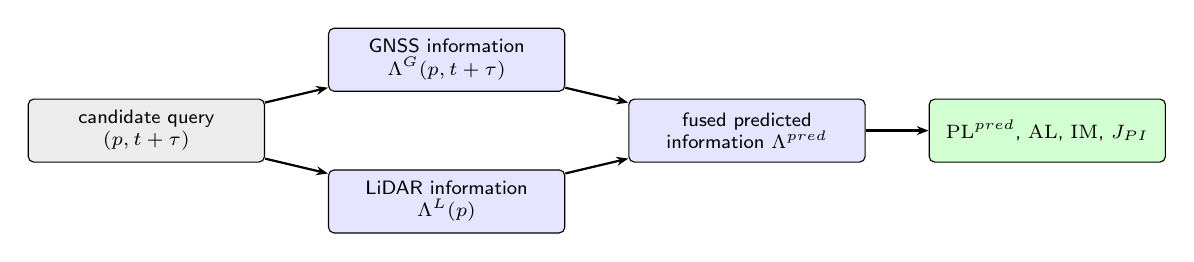
\begin{tikzpicture}[
      node distance=5mm and 8mm,
      box/.style={draw,rounded corners=2pt,minimum width=30mm,minimum height=8mm,font=\scriptsize,align=center},
      inputbox/.style={box,fill=gray!15},
      proc/.style={box,fill=blue!10},
      outputbox/.style={box,fill=green!18},
      arr/.style={-{Stealth[length=1.5mm]},thick}
    ]
    \node[inputbox] (q) {candidate query\\$(p,t+\tau)$};
    \node[proc,right=of q,yshift=9mm] (gnss) {GNSS information\\$\Lambda^G(p,t+\tau)$};
    \node[proc,right=of q,yshift=-9mm] (lidar) {LiDAR information\\$\Lambda^L(p)$};
    \node[proc,right=of gnss,yshift=-9mm] (fusion) {fused predicted\\information $\Lambda^{pred}$};
    \node[outputbox,right=of fusion] (pl) {$\PL^{pred}$, $\AL$, $\IM$, $J_{PI}$};
    \draw[arr] (q) -- (gnss);
    \draw[arr] (q) -- (lidar);
    \draw[arr] (gnss) -- (fusion);
    \draw[arr] (lidar) -- (fusion);
    \draw[arr] (fusion) -- (pl);
  \end{tikzpicture}

  \vspace{8pt}
  \begin{block}{Core idea}
    \footnotesize The predictor estimates how much future GNSS and LiDAR information would be available at a candidate location, then converts the fused information into a predicted position-domain PL.
  \end{block}
\end{frame}

\begin{frame}{3.3.3 GNSS Predictor: Geometry and Effective Measurement Variance}
  \small
  \begin{block}{GNSS geometry matrix at candidate position $p$}
    % \vspace{-4pt}
    \[
      G(p,t)=
      \begin{bmatrix}
        -e_1^\top & 1\\
        -e_2^\top & 1\\
        \vdots & \vdots\\
        -e_N^\top & 1
      \end{bmatrix},\qquad
      e_s=\frac{p^W_s(t)-p}{\|p^W_s(t)-p\|}.
    \]
  \end{block}

  \begin{block}{Predicted effective pseudorange variance}
    % \vspace{-4pt}
    \[
      \sigma^2_{eff,s}(p,t)=
      \sigma^2_{URE,s}+\sigma^2_{tropo,s}+\sigma^2_{iono,s}
      +\sigma^2_{mp}(el_s)+\sigma^2_{env}(p,el_s,az_s).
    \]
  \end{block}

  \begin{table}\scriptsize
    \begin{tabular}{p{0.20\textwidth} p{0.72\textwidth}}
      \toprule
      \textbf{Symbol} & \textbf{Meaning}\\
      \midrule
      $e_s$ & Unit line-of-sight vector from candidate position $p$ to satellite $s$.\\
      $N$ & Number of predicted visible satellites.\\
      $el_s,az_s$ & Elevation and azimuth of satellite $s$ as seen from $p$.\\
      $\sigma_{URE,s}$ & User range error standard deviation.\\
      $\sigma_{env}$ & Environment-dependent degradation, e.g., canopy, urban canyon, NLOS risk.\\
      \bottomrule
    \end{tabular}
  \end{table}
\end{frame}

\begin{frame}{3.3.4 GNSS Predictor: Information and Expected PL Proxy}
  \small
  \begin{block}{Predicted GNSS information}
    % \vspace{-4pt}
    \[
      W^G(p,t)=\diag\left(\sigma^{-2}_{eff,1},\ldots,\sigma^{-2}_{eff,N}\right),
      \qquad
      \Lambda^G(p,t)=G(p,t)^\top W^G(p,t)G(p,t).
    \]
  \end{block}

  \begin{block}{Geometry-driven GNSS PL proxy}
    % \vspace{-4pt}
    \[
      \PL^{G,pred}_q(p,t)=
      K^G_q\sqrt{e_q^\top\left(\Lambda^G(p,t)+\Lambda^{prior}\right)^{-1}e_q}
      +b^G_q(p,t).
    \]
  \end{block}

  \begin{table}\scriptsize
    \begin{tabular}{p{0.20\textwidth} p{0.72\textwidth}}
      \toprule
      \textbf{Symbol} & \textbf{Meaning}\\
      \midrule
      $W^G$ & GNSS measurement weight matrix.\\
      $\Lambda^G$ & Predicted GNSS information matrix at query location.\\
      $\Lambda^{prior}$ & Current prior information propagated from the localization snapshot.\\
      $e_q$ & Unit vector selecting horizontal or vertical position direction.\\
      $K^G_q$ & Conservative multiplier used for advisory GNSS PL proxy.\\
      $b^G_q$ & Predicted GNSS bias overbound from multipath, NLOS, or environment risk.\\
      \bottomrule
    \end{tabular}
  \end{table}
\end{frame}

\begin{frame}[fragile]{3.3.4b Pseudo-Code: GNSS Advisory Predictor}
\begin{lstlisting}
Input:
  candidate position p
  prediction time t + tau
  satellite ephemeris / visible satellite set
  sky mask or canopy / obstruction model
  prior information Lambda_prior

1. Predict satellite positions at t + tau.
2. For each satellite s:
      compute line-of-sight vector e_s(p)
      predict elevation and azimuth
      estimate visibility probability v_s(p)
      estimate effective variance sigma_eff,s^2(p)
3. Build geometry matrix G(p,t).
4. Build weight matrix W(p,t).
5. Compute GNSS information: Lambda_G(p,t) = G^T W G.
6. Convert to advisory PL proxy if needed:
      PL_G_pred = K sqrt(e_q^T (Lambda_prior + Lambda_G)^-1 e_q) + b_G
7. Return Lambda_G and PL_G_pred.
\end{lstlisting}
\end{frame}

\begin{frame}[fragile]{Illustration of GNSS Advisory Predictor Field}
\begin{figure}
    \centering
    
\includegraphics[width=0.85\linewidth]{pics/10.png}
    \label{fig:placeholder}
\end{figure}
\end{frame}

\begin{frame}{3.3.5 LiDAR Predictor: From Distance Heuristic to Observability FIM}
  \small
  \begin{alertblock}{Weakness of the previous design}
    \footnotesize A rule like ``farther point cloud means lower confidence'' is not a sufficient LiDAR integrity model. LiDAR integrity depends on geometric observability, map consistency, overlap, degeneracy, and feature distribution.
  \end{alertblock}

  \begin{block}{Predicted LiDAR information at candidate position $p$}
    % \vspace{-4pt}
    \[
      \Lambda^L(p)=\sum_{i\in\mathcal{V}_L(p)}\pi_i(p)J_i(p)^\top R_i(p)^{-1}J_i(p).
    \]
  \end{block}

  \begin{table}\scriptsize
    \begin{tabular}{p{0.22\textwidth} p{0.70\textwidth}}
      \toprule
      \textbf{Symbol} & \textbf{Meaning}\\
      \midrule
      $\mathcal{V}_L(p)$ & Predicted visible LiDAR features / voxels from candidate position $p$.\\
      $J_i(p)$ & Jacobian of the LiDAR residual associated with feature $i$.\\
      $R_i(p)$ & Measurement covariance including range noise, normal uncertainty, incidence angle, and map freshness.\\
      $\pi_i(p)$ & Visibility / overlap probability of feature $i$ from $p$.\\
      $\Lambda^L(p)$ & Predicted LiDAR Fisher information / observability matrix.\\
      \bottomrule
    \end{tabular}
  \end{table}
\end{frame}

\begin{frame}{3.3.6 LiDAR Predictor: TDOP and Feature Diversity}
  \small
  \begin{block}{Tree / feature dilution of precision}
    % \vspace{-4pt}
    \[
      G_{tree}(p)=
      \begin{bmatrix}
        \nu_1^\top\\ \nu_2^\top\\ \vdots\\ \nu_K^\top
      \end{bmatrix},\qquad
      \nu_k=\frac{c_k-p_{xy}}{\|c_k-p_{xy}\|}.
    \]
    \[
      TDOP(p)=\sqrt{\tr\left((G_{tree}(p)^\top W_{tree}(p)G_{tree}(p))^{-1}\right)}.
    \]
  \end{block}
\vspace{-2mm}
  \begin{table}\scriptsize
    \begin{tabular}{p{0.20\textwidth} p{0.72\textwidth}}
      \toprule
      \textbf{Symbol} & \textbf{Meaning}\\
      \midrule
      $c_k$ & Horizontal center of trunk / geometric landmark $k$.\\
      $p_{xy}$ & Horizontal component of candidate UAV position $p$.\\
      $\nu_k$ & Unit direction from candidate position to landmark $k$.\\
      $K$ & Number of predicted visible geometric landmarks.\\
      $W_{tree}$ & Weight matrix from trunk detection quality, distance, and map confidence.\\
      $TDOP$ & Tree dilution of precision; lower value means stronger geometric diversity.\\
      \bottomrule
    \end{tabular}
  \end{table}
\vspace{-2mm}

  \begin{exampleblock}{Interpretation}
    \footnotesize Features concentrated in one direction give weak geometry. Features surrounding the UAV give strong LiDAR observability.
  \end{exampleblock}
\end{frame}

\begin{frame}[fragile]{Illustration of LiDAR Observability / FIM Predictor}
\begin{figure}
    \centering
    
\includegraphics[width=0.95\linewidth]{pics/11.png}
    \label{fig:placeholder}
\end{figure}
\end{frame}

\begin{frame}{3.3.7 LiDAR Predicted PL}
  \small
  \begin{block}{LiDAR predicted PL proxy}
    % \vspace{-4pt}
    \[
      \PL^{L,pred}_q(p)=
      K^L_q\sqrt{e_q^\top\left(\Lambda^{prior}+\Lambda^L(p)\right)^{-1}e_q}+b^L_q(p).
    \]
  \end{block}

  \begin{block}{LiDAR bias / degradation overbound}
    % \vspace{-4pt}
    \[
      b^L_q(p)=\beta_1R_{map}(p)+\beta_2R_{dyn}(p)+\beta_3R_{overlap}(p)+\beta_4R_{deg}(p)+\beta_5R_{inc}(p).
    \]
  \end{block}

  \begin{table}\scriptsize
    \begin{tabular}{p{0.21\textwidth} p{0.70\textwidth}}
      \toprule
      \textbf{Symbol} & \textbf{Meaning}\\
      \midrule
      $K^L_q$ & Conservative multiplier for LiDAR advisory PL.\\
      $R_{map}$ & Map freshness / map-age risk.\\
      $R_{dyn}$ & Dynamic-object contamination risk.\\
      $R_{overlap}$ & Low source-target overlap risk.\\
      $R_{deg}$ & Geometric degeneracy risk, e.g., planar or corridor-like structure.\\
      $R_{inc}$ & Incidence-angle or grazing-view risk.\\
      $\beta_i$ & Calibration coefficients converting each risk term to a meter-level bias bound.\\
      \bottomrule
    \end{tabular}
  \end{table}
\end{frame}

\begin{frame}[fragile]{3.3.7b Pseudo-Code: LiDAR Observability Predictor}
\begin{lstlisting}
Input:
  candidate position p
  local feature / voxel map
  voxel normal statistics
  map age and dynamic probability
  prior information Lambda_prior

1. Query nearby candidate features / voxels V(p).
2. For each feature i in V(p):
      estimate visibility probability pi_i(p)
      compute residual Jacobian J_i(p)
      build measurement covariance R_i(p)
      apply map age / degeneracy inflation
      accumulate information: Lambda_L += pi_i J_i^T R_i^-1 J_i
3. Compute observability diagnostics:
      normal diversity, condition number, TDOP / LDOP
4. Compute bias overbound b_L(p).
5. Compute LiDAR advisory PL:
      PL_L_pred = K sqrt(e_q^T (Lambda_prior + Lambda_L)^-1 e_q) + b_L
6. Return Lambda_L, PL_L_pred, diagnostics.
\end{lstlisting}
\end{frame}

\begin{frame}{3.3.8 Fusion Predictor: Unified Future Information}
  \small
  \begin{block}{Unified predicted information}
    % \vspace{-4pt}
    \[
      \Lambda^{pred}(p,t+\tau)=\Lambda^{prior}(t+\tau)+\Lambda^G(p,t+\tau)+\Lambda^L(p).
    \]
  \end{block}

  \begin{block}{Predicted PL under advisory fault / degradation modes}
    % \vspace{-4pt}
    \[
      \PL^{pred}_q(p,t+\tau)=
      \max_{f\in\Hset^{pred}}
      \left(
        K_{f,q}\sqrt{e_q^\top\left(\Lambda^{pred}_f(p,t+\tau)\right)^{-1}e_q}
        +b_{f,q}(p,t+\tau)
      \right).
    \]
  \end{block}

  \begin{table}\scriptsize
    \begin{tabular}{p{0.23\textwidth} p{0.68\textwidth}}
      \toprule
      \textbf{Symbol} & \textbf{Meaning}\\
      \midrule
      $\Lambda^{prior}$ & Propagated current localization information before adding future measurements.\\
      $\Lambda^G$ & Predicted GNSS information at candidate position and time.\\
      $\Lambda^L$ & Predicted LiDAR information at candidate position.\\
      $\Hset^{pred}$ & Advisory degradation modes, e.g., GNSS weak geometry, LiDAR low observability, or source dominance.\\
      $\Lambda^{pred}_f$ & Predicted information matrix under mode $f$.\\
      $b_{f,q}$ & Predicted bias/degradation overbound under mode $f$.\\
      \bottomrule
    \end{tabular}
  \end{table}
\end{frame}

\begin{frame}[fragile]{3.3.8b Pseudo-Code: Advisory GNSS--LiDAR Fusion}
\begin{lstlisting}
Input:
  Lambda_prior
  Lambda_G(p,t)
  Lambda_L(p,t)
  advisory degradation modes
  alert limit AL(p)

1. Fuse information:
      Lambda_pred = Lambda_prior + Lambda_G + Lambda_L
2. For each advisory degradation mode f:
      modify Lambda_pred,f or bias b_f
      compute Sigma_pred,f = Lambda_pred,f^{-1}
      compute PL_f
3. Take worst case:
      PL_pred = max_f PL_f
4. Compute:
      IM = AL - PL_pred
      c_PI = margin_to_cost(IM)
5. Return PL_pred, IM, c_PI.
\end{lstlisting}
\end{frame}

\begin{frame}[fragile]{Illustration of GNSS--LiDAR Complementarity for Advisory Planning}
\begin{figure}
    \centering
    
\includegraphics[width=0.9\linewidth]{pics/12.png}
    \label{fig:placeholder}
\end{figure}
\end{frame}

\begin{frame}{3.3.9 Alert Limit, Integrity Margin, and PI Cost}
  \small
    \vspace{-2mm}
  
  \begin{columns}[T]
    \column{0.48\textwidth}
    \begin{block}{Environment-side alert limit}
      % \vspace{-4pt}
      \[
        \AL(p)=\min\left(\gamma_H d_{obs}(p),\ \gamma_V d_{vertical}(p)\right).
      \]
    \end{block}

    \column{0.48\textwidth}
    \begin{block}{Integrity margin}
      % \vspace{-4pt}
      \[
        \IM(p,t)=\AL(p)-\PL^{pred}(p,t).
      \]
    \end{block}
  \end{columns}
    \vspace{-1mm}

  \vspace{3pt}
  \begin{exampleblock}{Planner-compatible PI cost}
    % \vspace{-2pt}
    \[
      \begin{aligned}
        J_{PI}(p,t)&=\lambda_r\,[\PL^{pred}(p,t)-\AL(p)+m]^2_+\\
        &\quad+\lambda_{ratio}\left(\frac{\PL^{pred}(p,t)}{\AL(p)+\epsilon}\right)^2.
      \end{aligned}
    \]
  \end{exampleblock}
    \vspace{-2mm}

  \begin{table}\scriptsize
    \begin{tabular}{p{0.18\textwidth} p{0.75\textwidth}}
      \toprule
      \textbf{Symbol} & \textbf{Meaning}\\
      \midrule
      $d_{obs}(p)$ & ESDF obstacle clearance at position $p$.\\
      $d_{vertical}(p)$ & Vertical clearance to altitude bounds or canopy boundary.\\
      $\gamma_H,\gamma_V$ & Safety factors mapping clearance to horizontal and vertical alert limits.\\
      $m$ & Extra integrity margin requested by the planner.\\
      $[a]_+=\max(a,0)$ & Hinge operator. It penalizes only unsafe or near-unsafe margin.\\
      $\lambda_r,\lambda_{ratio}$ & Weights for hard-margin risk and soft preference.\\
      \bottomrule
    \end{tabular}
  \end{table}
\end{frame}

\begin{frame}{3.3.10 Predictor Module Summary}
  \small
  \begin{columns}[T]
    \column{0.50\textwidth}
    \textbf{Method flow}
    \begin{enumerate}\footnotesize
      \item Query candidate position $p$ and future time $t+\tau$.
      \item Predict GNSS information from satellite visibility and variance.
      \item Predict LiDAR information from feature observability and FIM.
      \item Fuse information into $\Lambda^{pred}$.
      \item Convert to $\PL^{pred}$, $\AL$, $\IM$, and $J_{PI}$.
    \end{enumerate}

    \column{0.48\textwidth}
    \textbf{Main innovations}
    \begin{itemize}\footnotesize
      \item Future GNSS model is defined as advisory geometry-risk PL proxy.
      \item LiDAR predictor is upgraded from range heuristic to observability FIM.
      \item GNSS-LiDAR complementarity is handled by information fusion.
      \item Output is a unified cost, not two incompatible source-specific scores.
    \end{itemize}
  \end{columns}
\end{frame}

% ==================================================================
% \section{Ch3.4 Predicted PL Map Construction and Planner Interface}
% ==================================================================

\begin{frame}{3.4.0 PL Map Builder: Design Rationale}

  \small
  \begin{columns}[T]
    \column{0.48\textwidth}
    \begin{alertblock}{Previous weakness}
      \footnotesize
      A predictor query model is not directly usable by a high-rate planner. Recomputing prediction inside A* or B-spline optimization would duplicate computation and create synchronization problems.
    \end{alertblock}
    \column{0.49\textwidth}
    \begin{exampleblock}{Design idea}
      \footnotesize
      Build a rolling, cached, multi-layer Unified Risk Grid (URG). The map builder samples active voxels, stores $\PL^{pred}$, $\AL$, $\IM$, $c_{PI}$, age, and flags, then serves the same field to A* and B-spline.
    \end{exampleblock}
  \end{columns}
  \begin{block}{Benefit / innovation}
    \footnotesize Prediction becomes an asynchronous map-generation process rather than a heavy per-query planner computation.
  \end{block}

\end{frame}

\begin{frame}{3.4.1 Why We Need a PL Map Construction Layer}
  \small
  \begin{block}{Predictor vs map builder}
    \vspace{-4pt}
    \[
      \text{Predictor model: } f_{pred}(p,t)\quad\Longrightarrow\quad
      \text{Map builder: sample } f_{pred} \text{ over active voxels.}
    \]
  \end{block}

  \begin{columns}[T]
    \column{0.48\textwidth}
    \textbf{Predictor}
    \begin{itemize}\footnotesize
      \item Continuous or discrete query model.
      \item Input: one candidate position and time.
      \item Output: predicted PL / AL / IM / PI cost for that query.
    \end{itemize}

    \column{0.48\textwidth}
    \textbf{PL map builder}
    \begin{itemize}\footnotesize
      \item Batched sampler and cache manager.
      \item Input: active voxel set.
      \item Output: rolling local multi-layer map queried by A* and B-spline.
    \end{itemize}
  \end{columns}

  \begin{alertblock}{Important distinction}
    \footnotesize Mathematically, the PL map samples predictor values per voxel. Engineering-wise, it should not run a full heavy ARAIM pipeline for every voxel.
  \end{alertblock}
\end{frame}

\begin{frame}{3.4.2 Rolling Local Grid Definition}
  \small
  \begin{block}{Local rolling grid centered around the UAV}
    % \vspace{-4pt}
    \[
      \Ggrid_t=\left\{p_i\;\middle|\;
        \begin{array}{l}
          p_i\in [x_t-L_x,x_t+L_x]\times[y_t-L_y,y_t+L_y]\\
          \qquad\quad\times[z_t-L_z,z_t+L_z],\quad p_i\ \text{is a voxel center}
        \end{array}
      \right\}.
    \]
  \end{block}

  \begin{block}{Multi-layer value stored at each voxel}
    % \vspace{-1pt}
    \[
      \Mmap_{PL}(p_i)=\{\PL^{G,pred}_i,\PL^{L,pred}_i,\PL^{fused,pred}_i,\AL_i,\IM_i,J_{PI,i},stamp_i\}.
    \]
  \end{block}

  \begin{table}\scriptsize
    \begin{tabular}{p{0.20\textwidth} p{0.72\textwidth}}
      \toprule
      \textbf{Symbol} & \textbf{Meaning}\\
      \midrule
      $L_x,L_y,L_z$ & Half-size of the rolling local prediction box.\\
      $p_i$ & Center of voxel $i$.\\
      $stamp_i$ & Last update time of the voxel; used for staleness checking.\\
      $\Mmap_{PL}$ & Predicted PL/AL/IM/cost map used by planning.\\
      \bottomrule
    \end{tabular}
  \end{table}
\end{frame}

\begin{frame}{3.4.3 Per-Voxel Prediction Pipeline}
  \small
  \begin{block}{For each active voxel $p_i$}
    % \vspace{-4pt}
    \[
      \Lambda^{pred}_i=\Lambda^{prior}+\Lambda^G(p_i,t+\tau_i)+\Lambda^L(p_i),
    \]
    \[
      \PL^{pred}_i=K_i\sqrt{e_q^\top(\Lambda^{pred}_i)^{-1}e_q}+b_i,
      \qquad
      \IM_i=\AL_i-\PL^{pred}_i.
    \]
  \end{block}

  \begin{block}{Planner cost layer}
    % \vspace{-4pt}
    \[
      J_{PI,i}=\lambda_r[\PL^{pred}_i-\AL_i+m]^2_+
      +\lambda_{ratio}\left(\frac{\PL^{pred}_i}{\AL_i+\epsilon}\right)^2.
    \]
  \end{block}

  \begin{table}\scriptsize
    \begin{tabular}{p{0.22\textwidth} p{0.68\textwidth}}
      \toprule
      \textbf{Variable} & \textbf{Meaning}\\
      \midrule
      $\tau_i$ & Prediction horizon associated with voxel $p_i$; may be constant or estimated from path progress.\\
      $\Lambda^{pred}_i$ & Predicted fused information at voxel $i$.\\
      $K_i,b_i$ & Conservative multiplier and bias overbound for voxel $i$.\\
      $J_{PI,i}$ & Scalar cost consumed by A* and trajectory optimization.\\
      \bottomrule
    \end{tabular}
  \end{table}
\end{frame}

\begin{frame}[fragile]{3.4.3b Pseudo-Code: Rolling Predicted PL Map Construction}
\begin{lstlisting}
Input:
  rolling grid G_t
  current snapshot S_t
  cached GNSS / LiDAR information fields
  ESDF / occupancy map

For each active voxel p_i in G_t:
    if occupied or outside planning bounds:
        mark infeasible
        continue
    AL_i = compute_alert_limit_from_ESDF(p_i)
    Lambda_G_i = query_or_compute_GNSS_information(p_i)
    Lambda_L_i = query_or_compute_LiDAR_information(p_i)
    Lambda_pred_i = Lambda_prior + Lambda_G_i + Lambda_L_i
    PL_i = compute_advisory_PL_proxy(Lambda_pred_i, bias_i)
    IM_i = AL_i - PL_i
    c_PI_i = margin_to_cost(PL_i, AL_i)
    write layers: PL, AL, IM, c_PI, age, flags

Rule: sample active voxels; do not run full ARAIM per voxel.
\end{lstlisting}
\end{frame}

\begin{frame}[fragile]{Illustration of Predicted PL Map Construction}
\begin{figure}
    \centering
    
\includegraphics[width=0.9\linewidth]{pics/13.png}
    \label{fig:placeholder}
\end{figure}
\end{frame}

\begin{frame}{3.4.4 Active Voxels: Avoid Computing the Whole Box Every Time}
  \small
  \begin{columns}[T]
    \column{0.48\textwidth}
    \begin{block}{Full-grid mode}
      \footnotesize
      Used for debugging and visualization.
      \[
        N_{vox}\approx \frac{2L_x}{r}\frac{2L_y}{r}\frac{2L_z}{r}.
      \]
      For example, $30\,m\times30\,m\times8\,m$ at $1\,m$ resolution gives about $7200$ voxels.
    \end{block}

    \column{0.48\textwidth}
    \begin{exampleblock}{Active-voxel mode}
      \footnotesize
      Used for online planning.
      \begin{itemize}\scriptsize
        \item Free voxels only.
        \item Current local corridor around the nominal path.
        \item A* search frontier or visited nodes.
        \item B-spline trajectory samples and neighbors.
        \item High-risk boundary region from previous map.
      \end{itemize}
    \end{exampleblock}
  \end{columns}

  \begin{alertblock}{Engineering rule}
    \footnotesize The map builder samples a cached lightweight advisory model over active voxels, rather than executing full ARAIM per voxel.
  \end{alertblock}
\end{frame}

\begin{frame}{3.4.5 Shared Multi-Layer Map}
  \small
  \begin{block}{Unified map data structure}
    % \vspace{-4pt}
    \[
      \Mmap(p)=\{\Occ(p),\ESDF(p),\AL(p),\Lambda^G(p),\Lambda^L(p),\PL^{pred}(p),\IM(p),J_{PI}(p)\}.
    \]
  \end{block}

  \begin{table}\scriptsize
    \begin{tabular}{p{0.23\textwidth} p{0.25\textwidth} p{0.40\textwidth}}
      \toprule
      \textbf{Layer} & \textbf{Source} & \textbf{Used by}\\
      \midrule
      $\Occ$ & LiDAR occupancy map & A* hard collision check\\
      $\ESDF$ & Occupancy distance transform & A*, B-spline obstacle gradient, AL\\
      $\AL$ & ESDF and flight bounds & PI function\\
      $\Lambda^G$ & GNSS visibility and geometry & GNSS predictor\\
      $\Lambda^L$ & LiDAR observability field & LiDAR predictor\\
      $\PL^{pred}$ & Fused advisory prediction & A*, B-spline, visualization\\
      $\IM$ & $\AL-\PL^{pred}$ & Safety margin analysis\\
      $J_{PI}$ & Margin-to-cost transform & Planning optimization\\
      \bottomrule
    \end{tabular}
  \end{table}

  \begin{block}{Key message}
    \footnotesize The A* map and PL field are merged as layers of one map, but occupancy, ESDF, PL, and cost must keep separate semantics.
  \end{block}
\end{frame}

\begin{frame}[fragile]{Illustration of Unified Risk Grid (URG) Layers}
\begin{figure}
    \centering
    
\includegraphics[width=1.0\linewidth]{pics/14.png}
    \label{fig:placeholder}
\end{figure}
\end{frame}

\begin{frame}{3.4.6 Planner Query Interface}
  \small
  \begin{columns}[T]
    \column{0.48\textwidth}
    \begin{block}{A* front-end query}
      % \vspace{-4pt}
      \[
        c(e)=c_{dist}(e)+\lambda_{obs}c_{obs}(e)+\lambda_{PI}\sum_{p_i\in e}J_{PI}(p_i)\Delta s.
      \]
      \footnotesize A* queries discrete voxel values along graph edges.
    \end{block}

    \column{0.48\textwidth}
    \begin{exampleblock}{B-spline back-end query}
      % \vspace{-4pt}
      \[
        \begin{aligned}
          J^{traj}_{PI}&=\sum_k J_{PI}(p(t_k)),\\
          J_{PI}(p)&=\Interp(\Mmap_{PI},p).
        \end{aligned}
      \]
      \footnotesize The optimizer queries a continuous field by trilinear interpolation.
    \end{exampleblock}
  \end{columns}

  \begin{table}\scriptsize
    \begin{tabular}{p{0.18\textwidth} p{0.74\textwidth}}
      \toprule
      \textbf{Symbol} & \textbf{Meaning}\\
      \midrule
      $e$ & A* graph edge between two neighboring nodes.\\
      $c_{dist}$ & Geometric edge length cost.\\
      $c_{obs}$ & Obstacle clearance cost from occupancy / ESDF.\\
      $\Delta s$ & Edge sampling interval.\\
      $p(t_k)$ & Sampled point on the continuous B-spline trajectory.\\
      $\Interp$ & Trilinear interpolation from voxel field to continuous position.\\
      \bottomrule
    \end{tabular}
  \end{table}
\end{frame}

\begin{frame}{3.4.7 Caching, Staleness, and Runtime Scheduling}
  \small
  \begin{table}\scriptsize
    \begin{tabular}{p{0.35\textwidth} p{0.22\textwidth} p{0.33\textwidth}}
      \toprule
      \textbf{Component} & \textbf{Suggested rate} & \textbf{Notes}\\
      \midrule
      LiDAR occupancy / ESDF update & 5--20 Hz & High-rate mapping and obstacle safety.\\
      Current ARAIM monitor & 5--10 Hz & Current PL and alarm supervision.\\
      Advisory PL map update & 1--2 Hz & Expensive; use active voxels and cache.\\
      A* local replan & 5--10 Hz & Uses latest non-stale cost field.\\
      B-spline back-end optimization & 10--50 Hz & Uses interpolation and finite/analytic gradients.\\
      \bottomrule
    \end{tabular}
  \end{table}

  \begin{block}{Staleness check}
    \vspace{-4pt}
    \[
      \text{valid}(p_i)=\left(t_{now}-stamp_i\le T_{max\_age}\right)\land\left(p_i\in\Ggrid_t\right).
    \]
  \end{block}

  \begin{alertblock}{Fallback logic}
    \footnotesize If the PL/cost field is stale or unavailable, the planner falls back to standard collision-aware EGO behavior, while current ARAIM remains active for supervision.
  \end{alertblock}
\end{frame}

\begin{frame}{3.4.8 PL Map Construction Summary}
  \small
  \begin{columns}[T]
    \column{0.50\textwidth}
    \textbf{Method flow}
    \begin{enumerate}\footnotesize
      \item Define rolling local grid and active voxel set.
      \item Query cached GNSS/LiDAR information fields.
      \item Fuse information and compute advisory PL.
      \item Compute AL, IM, and planner cost.
      \item Publish multi-layer map to A* and B-spline optimizer.
    \end{enumerate}

    \column{0.48\textwidth}
    \textbf{Main innovations}
    \begin{itemize}\footnotesize
      \item Predictor output becomes a reusable map, not a one-off scalar.
      \item A* and back-end share the same integrity field.
      \item Active-voxel update makes dense PL prediction tractable.
      \item Staleness and fallback keep the system robust.
    \end{itemize}
  \end{columns}
\end{frame}

% ==================================================================
% \section{Ch3.5 Integrity-Aware Planning}
% ==================================================================

\begin{frame}{3.5.0 Planning Module: Design Rationale}

  \small
  \begin{columns}[T]
    \column{0.48\textwidth}
    \begin{alertblock}{Previous weakness}
      \footnotesize
      A collision-free path can still be localization-unsafe. If A* and the back-end query inconsistent risk fields, the optimized trajectory may fight the front-end initialization.
    \end{alertblock}
    \column{0.49\textwidth}
    \begin{exampleblock}{Design idea}
      \footnotesize
      Use one planner-compatible integrity scalar derived from the predicted integrity margin:
      \[
        \IM(p,t)=\AL(p)-\PL^{pred}(p,t),\qquad c_{PI}=\phi(\IM).
      \]
      Both A* and B-spline query this same cost layer.
    \end{exampleblock}
  \end{columns}
  \begin{block}{Benefit / innovation}
    \footnotesize The front-end produces an integrity-aware initial path and the back-end refines it with the same semantic cost field.
  \end{block}

\end{frame}

\begin{frame}{3.5.1 Planning Module Overview}
  \small
  \begin{block}{Input-output contract}
    \vspace{-4pt}
    \[
      \left(\Mmap_{occ},\Mmap_{ESDF},\Mmap_{PI},\hat{x}_t,p_{goal}\right)
      \longrightarrow
      \tau(t)=\text{safe and integrity-aware trajectory}.
    \]
  \end{block}

  \begin{columns}[T]
    \column{0.48\textwidth}
    \textbf{A* front-end}
    \begin{itemize}\footnotesize
      \item Searches a collision-free initial path.
      \item Uses PI cost to avoid low-integrity regions early.
      \item Provides a topologically reasonable initialization.
    \end{itemize}

    \column{0.48\textwidth}
    \textbf{B-spline back-end}
    \begin{itemize}\footnotesize
      \item Optimizes smoothness, dynamics, obstacle clearance, and PI cost.
      \item Queries continuous PI field by interpolation.
      \item Produces controller-ready trajectory.
    \end{itemize}
  \end{columns}
\end{frame}

\begin{frame}{3.5.2 Integrity-Aware A* Front-End}
  \small
  \begin{block}{Edge cost used by A*}
    \vspace{-4pt}
    \[
      c(e)=w_d\,c_{dist}(e)+w_o\,c_{obs}(e)+w_I\,c_{int}(e),
    \]
    \[
      c_{int}(e)=\sum_{p_i\in\mathrm{Sample}(e)}J_{PI}(p_i)\Delta s.
    \]
  \end{block}

  \begin{table}\scriptsize
    \begin{tabular}{p{0.20\textwidth} p{0.72\textwidth}}
      \toprule
      \textbf{Variable} & \textbf{Meaning}\\
      \midrule
      $c_{dist}$ & Euclidean edge length or traversal distance.\\
      $c_{obs}$ & Obstacle-related cost; infinite or very large if the edge is in occupied space.\\
      $c_{int}$ & Accumulated integrity cost along the edge.\\
      $w_d,w_o,w_I$ & Weights for distance, obstacle, and integrity terms.\\
      $\mathrm{Sample}(e)$ & Sampled voxel centers or interpolation points along edge $e$.\\
      \bottomrule
    \end{tabular}
  \end{table}

  \begin{exampleblock}{Innovation}
    \footnotesize A* is upgraded from ``collision-free search'' to ``collision-free and integrity-aware initial path search''.
  \end{exampleblock}
\end{frame}

\begin{frame}{3.5.3 Why A* Needs the PL Map}
  \small
  \begin{columns}[T]
    \column{0.48\textwidth}
    \begin{alertblock}{Without PL map}
      \footnotesize A* only sees occupancy / ESDF. It cannot distinguish two obstacle-free routes with different localization integrity.
    \end{alertblock}

    \textbf{Failure mode}
    \begin{itemize}\footnotesize
      \item Initial path may enter GNSS-shadowed or LiDAR-degenerate area.
      \item Back-end receives a poor initialization.
      \item PI gradient may be too local to escape the bad corridor.
    \end{itemize}

    \column{0.48\textwidth}
    \begin{exampleblock}{With PL map}
      \footnotesize A* sees both collision risk and localization-integrity risk.
    \end{exampleblock}

    \textbf{Benefit}
    \begin{itemize}\footnotesize
      \item Initial path avoids high-PL regions.
      \item Back-end starts in a better basin.
      \item Planning becomes proactive instead of alarm-reactive.
    \end{itemize}
  \end{columns}
\end{frame}

\begin{frame}{3.5.4 B-spline Back-End Objective}
  \small
  \begin{block}{Control-point optimization problem}
    % \vspace{-4pt}
    \[
      \min_{\mathbf{Q}}\quad
      J(\mathbf{Q})=
      \lambda_sJ_{smooth}(\mathbf{Q})
      +\lambda_dJ_{dyn}(\mathbf{Q})
      +\lambda_oJ_{obs}(\mathbf{Q})
      +\lambda_IJ_{PI}^{traj}(\mathbf{Q}).
    \]
  \end{block}

  \begin{table}\scriptsize
    \begin{tabular}{p{0.20\textwidth} p{0.72\textwidth}}
      \toprule
      \textbf{Symbol} & \textbf{Meaning}\\
      \midrule
      $\mathbf{Q}=\{Q_0,\ldots,Q_M\}$ & B-spline control points.\\
      $J_{smooth}$ & Smoothness cost, usually based on acceleration / jerk / snap derivatives.\\
      $J_{dyn}$ & Dynamic feasibility cost, e.g., velocity and acceleration limits.\\
      $J_{obs}$ & Obstacle avoidance cost from ESDF.\\
      $J_{PI}^{traj}$ & Integrity-aware trajectory cost sampled along the continuous trajectory.\\
      $\lambda_s,\lambda_d,\lambda_o,\lambda_I$ & Weights for smoothness, dynamics, obstacle, and integrity terms.\\
      \bottomrule
    \end{tabular}
  \end{table}
\end{frame}

\begin{frame}{3.5.5 B-spline Trajectory and PI Cost Sampling}
  \small
  \begin{block}{B-spline position trajectory}
    % \vspace{-4pt}
    \[
      p(t)=\sum_{i=0}^{M}B_i^k(t)Q_i.
    \]
  \end{block}

  \begin{block}{Integrity cost along the trajectory}
    % \vspace{-4pt}
    \[
      J_{PI}^{traj}(\mathbf{Q})=\sum_{r=1}^{N_s}J_{PI}\left(p(t_r),t_r\right)\Delta t_r,
      \qquad
      J_{PI}(p)=\Interp(\Mmap_{PI},p).
    \]
  \end{block}

  \begin{table}\scriptsize
    \begin{tabular}{p{0.20\textwidth} p{0.72\textwidth}}
      \toprule
      \textbf{Symbol} & \textbf{Meaning}\\
      \midrule
      $B_i^k(t)$ & B-spline basis function of degree/order $k$ associated with control point $Q_i$.\\
      $Q_i$ & Spatial control point.\\
      $t_r$ & Trajectory sample time.\\
      $N_s$ & Number of sampled points for continuous-time cost approximation.\\
      $\Mmap_{PI}$ & Cached PI cost layer from the predicted PL map.\\
      \bottomrule
    \end{tabular}
  \end{table}
\end{frame}

\begin{frame}[fragile]{3.5.5b Pseudo-Code: Planner Query over Unified Risk Grid}
\begin{lstlisting}
A* front-end:
  for each expanded node p_j:
      check occupancy / ESDF
      query c_PI(p_j) from URG
      edge_cost = distance * (1 + lambda_obs c_obs + lambda_PI c_PI)

B-spline back-end:
  for each sampled trajectory point p(t_k):
      query ESDF gradient from URG
      query PI cost by trilinear interpolation from URG
      add obstacle and integrity cost

Reason:
  front-end and back-end query the same unified risk grid.
\end{lstlisting}
\end{frame}

\begin{frame}{3.5.6 Gradient for Back-End Optimization}
  \small
  \begin{block}{Chain rule from map cost to control point}
    % \vspace{-4pt}
    \[
      \frac{\partial J_{PI}^{traj}}{\partial Q_i}
      =\sum_{r=1}^{N_s}
      \frac{\partial J_{PI}(p(t_r))}{\partial p}
      \frac{\partial p(t_r)}{\partial Q_i}\Delta t_r
      =\sum_{r=1}^{N_s}
      \nabla_pJ_{PI}(p(t_r))B_i^k(t_r)\Delta t_r.
    \]
  \end{block}

  \begin{table}\scriptsize
    \begin{tabular}{p{0.22\textwidth} p{0.70\textwidth}}
      \toprule
      \textbf{Symbol} & \textbf{Meaning}\\
      \midrule
      $\nabla_pJ_{PI}(p)$ & Spatial gradient of the PI cost field, computed by finite difference or interpolation gradient.\\
      $\partial p/\partial Q_i=B_i^k(t)$ & Local support of B-spline: only nearby control points affect $p(t)$.\\
      $\Delta t_r$ & Quadrature / sampling weight.\\
      \bottomrule
    \end{tabular}
  \end{table}

  \begin{exampleblock}{Innovation}
    \footnotesize The same predicted PL map gives both a scalar cost and a spatial gradient for smooth trajectory optimization.
  \end{exampleblock}
\end{frame}

\begin{frame}{3.5.7 Safety Inequality Along the Planned Trajectory}
  \small
  \begin{block}{Integrity-aware safety condition}
    % \vspace{-4pt}
    \[
      \PL^{pred}(p(t),t)<\AL(p(t))\quad\Longleftrightarrow\quad \IM(p(t),t)>0.
    \]
  \end{block}

  \begin{block}{Soft constraint used by optimizer}
    % \vspace{-4pt}
    \[
      J_{violate}=\sum_{r=1}^{N_s}\left[\PL^{pred}(p(t_r),t_r)-\AL(p(t_r))+m\right]^2_+.
    \]
  \end{block}

  \begin{table}\scriptsize
    \begin{tabular}{p{0.20\textwidth} p{0.72\textwidth}}
      \toprule
      \textbf{Symbol} & \textbf{Meaning}\\
      \midrule
      $p(t)$ & Continuous planned trajectory position.\\
      $\PL^{pred}(p(t),t)$ & Predicted localization-side error bound along the trajectory.\\
      $\AL(p(t))$ & Environment-side tolerable position error at the same location.\\
      $m$ & Required safety margin beyond the strict $\PL<\AL$ inequality.\\
      \bottomrule
    \end{tabular}
  \end{table}
\end{frame}

\begin{frame}{3.5.8 Runtime and Unknown-Risk Fallback Logic}

  \small
  \begin{columns}[T]
    \column{0.50\textwidth}
    \begin{block}{Runtime policy}
      \footnotesize
      \begin{enumerate}
        \item Current ARAIM always supervises execution.
        \item PL map builder updates URG asynchronously.
        \item A* and B-spline query the latest valid URG.
        \item If the field is stale, trigger refresh or apply unknown-risk penalty.
      \end{enumerate}
    \end{block}
    \column{0.48\textwidth}
    \begin{alertblock}{Stale field is not safe field}
      \footnotesize
      \[
        c^{used}(p)=c_{PI}(p)+c_{unknown}(p)
      \]
      \[
        c_{unknown}(p)=\lambda_u\left(1-e^{-\Delta t(p)/\tau_u}\right).
      \]
      \scriptsize
      $\Delta t(p)$: field age at voxel $p$; $\lambda_u$: unknown-risk weight; $\tau_u$: aging time constant.
    \end{alertblock}
  \end{columns}
  \begin{exampleblock}{Fallback options}
    \footnotesize
    Trigger predictor refresh, slow down, conservatively replan, hover, or return depending on mission policy and current ARAIM alarm status.
  \end{exampleblock}

\end{frame}

\begin{frame}{3.5.9 Planning Module Summary}
  \small
  \begin{columns}[T]
    \column{0.50\textwidth}
    \textbf{Method flow}
    \begin{enumerate}\footnotesize
      \item Receive rolling multi-layer map.
      \item A* searches with distance, obstacle, and PI cost.
      \item B-spline refines the path using smoothness, dynamics, obstacle, and PI terms.
      \item Trajectory is sent to controller.
      \item Current ARAIM supervises execution.
    \end{enumerate}

    \column{0.48\textwidth}
    \textbf{Main innovations}
    \begin{itemize}\footnotesize
      \item A* uses predicted integrity, not only obstacles.
      \item Back-end cost has a direct PL/AL/IM interpretation.
      \item Same map supports front-end search and continuous optimization.
      \item Fallback keeps the system practical and safe.
    \end{itemize}
  \end{columns}
\end{frame}

% ==================================================================
% \section{Ch3.6 Innovation Summary and Next Implementation Plan}
% ==================================================================

\begin{frame}{3.6.1 Updated Methodology: Innovation Map}
  \small
  \begin{table}\scriptsize
    \begin{tabular}{p{0.22\textwidth} p{0.37\textwidth} p{0.33\textwidth}}
      \toprule
      \textbf{Module} & \textbf{Previous weakness} & \textbf{Updated innovation}\\
      \midrule
      Localization & Planner only consumed mean odometry. & Snapshot exposes covariance, GNSS epoch, and LiDAR factor blocks.\\
      Current ARAIM & GNSS and LiDAR PL were hard to combine; LiDAR PL could grow linearly. & Factor-block LiDAR ARAIM, bounded age risk, and conservative monitored fusion.\\
      Advisory predictor & Future GNSS/LiDAR PL models were too heuristic. & GNSS visibility/information model and LiDAR FIM/TDOP observability model.\\
      PL map & Predictor output was not clearly mapped to planner queries. & Rolling multi-layer PL/AL/IM/cost map with cache and staleness.\\
      Planning & Planner could not actively prefer high-integrity regions. & PI-aware A* initialization and B-spline back-end cost.\\
      \bottomrule
    \end{tabular}
  \end{table}
\end{frame}

% \begin{frame}{3.6.2 Implementation Priority}
%   \small
%   \begin{enumerate}\footnotesize
%     \item \textbf{Diagnose current LiDAR ARAIM PL growth}: log separation term, subset variance term, missed-detection margin, and bias term separately.
%     \item \textbf{Replace linear age penalty}: use bounded freshness risk and calibrate bias scale in meters.
%     \item \textbf{Implement information-domain fusion}: expose $\Lambda^G$, $\Lambda^L$, and fused $\Lambda^{pred}$.
%     \item \textbf{Upgrade GNSS predictor}: satellite visibility, sky mask / canopy model, effective variance, and geometry information.
%     \item \textbf{Upgrade LiDAR predictor}: feature observability, normal diversity, TDOP/FIM, overlap probability, and map freshness.
%     \item \textbf{Build rolling multi-layer PL map}: active voxel sampling, cache, staleness, planner interpolation query.
%     \item \textbf{Connect to planning}: PI-aware A* and back-end B-spline optimization using the same cost field.
%   \end{enumerate}
% \end{frame}

\begin{frame}{3.6.2 Validation Plan for the Updated Methodology}
  \small
  \begin{table}\scriptsize
    \begin{tabular}{p{0.23\textwidth} p{0.27\textwidth} p{0.38\textwidth}}
      \toprule
      \textbf{Test} & \textbf{Metric} & \textbf{Expected evidence}\\
      \midrule
      LiDAR ARAIM decomposition & $|d_f|$, $\sigma_f$, $b_f$, $\gamma_{age}$ & Verify whether PL growth comes from linear age bias or true observability loss.\\
      GNSS predictor sanity & Predicted satellite count, DOP, $\PL^{G,pred}$ & PL rises under canopy / canyon and decreases in open sky.\\
      LiDAR predictor sanity & TDOP/FIM, $\PL^{L,pred}$ & PL decreases in feature-rich and well-distributed geometry.\\
      Fusion behavior & $\PL^G,\PL^L,\PL^{fused}$ & Monitor keeps max fusion; advisory predictor uses FIM-add and is tested separately.\\
      Planner behavior & path length, minimum IM, collision clearance & A* and B-spline avoid low-integrity regions while keeping collision safety.\\
      Runtime & predictor latency, map update rate, planner rate & PL map updates asynchronously without blocking planning.\\
      \bottomrule
    \end{tabular}
  \end{table}
\end{frame}

\begin{frame}{3.6.3 Final Takeaway}
  \Large
  \begin{center}
    \textbf{The updated system is not just ``PL added to planning''.}
  \end{center}

  \vspace{8pt}
  \small
  \begin{block}{Core contribution}
    It builds a complete interface from sensor factors to current ARAIM, from advisory information prediction to a rolling PL map, and from that map to integrity-aware search and trajectory optimization.
  \end{block}

  \begin{exampleblock}{One-sentence summary}
    \centering
    \textbf{Current ARAIM monitors whether the UAV is safe now; advisory PL prediction helps the planner choose where it will remain safe in the future.}
  \end{exampleblock}
\end{frame}

\end{document}
